\documentclass[10pt,a4paper,oneside]{article}

% ---------------------------------------------------------------------------
% Preâmbulo base do repositório: fonte, mancha, pacotes, legenda, título e
% cabeçalho. Compile de dentro de `docs/product/`.
% ---------------------------------------------------------------------------
\usepackage[brazil]{babel}
% =====================================================================
%  Preâmbulo base: pacotes, tipografia e convenções de todo documento
%  LaTeX do repositório
%
%  Origem: `config/preambulo.tex` do documento de projeto do rhae-sensor.
%  As seções abaixo seguem a ordem de lá, e o que difere está marcado
%  com DIFERENÇA.
%
%  Convenções tipográficas e de apresentação adotadas
%    ISO 216        formato A4
%    ISO 80000-1    números e unidades (vírgula decimal, espaço fino entre
%                   grupos de três algarismos, unidade em tipo romano)
%    Tabelas sem filetes verticais (booktabs); legenda de tabela acima,
%    de figura abaixo.
%
%  Uso, antes do `\begin{document}`:
%    report/*.tex          via `\usepackage{estilo-reporte}`, que carrega este
%    docs/product/*.tex    % =====================================================================
%  Preâmbulo base: pacotes, tipografia e convenções de todo documento
%  LaTeX do repositório
%
%  Origem: `config/preambulo.tex` do documento de projeto do rhae-sensor.
%  As seções abaixo seguem a ordem de lá, e o que difere está marcado
%  com DIFERENÇA.
%
%  Convenções tipográficas e de apresentação adotadas
%    ISO 216        formato A4
%    ISO 80000-1    números e unidades (vírgula decimal, espaço fino entre
%                   grupos de três algarismos, unidade em tipo romano)
%    Tabelas sem filetes verticais (booktabs); legenda de tabela acima,
%    de figura abaixo.
%
%  Uso, antes do `\begin{document}`:
%    report/*.tex          via `\usepackage{estilo-reporte}`, que carrega este
%    docs/product/*.tex    % =====================================================================
%  Preâmbulo base: pacotes, tipografia e convenções de todo documento
%  LaTeX do repositório
%
%  Origem: `config/preambulo.tex` do documento de projeto do rhae-sensor.
%  As seções abaixo seguem a ordem de lá, e o que difere está marcado
%  com DIFERENÇA.
%
%  Convenções tipográficas e de apresentação adotadas
%    ISO 216        formato A4
%    ISO 80000-1    números e unidades (vírgula decimal, espaço fino entre
%                   grupos de três algarismos, unidade em tipo romano)
%    Tabelas sem filetes verticais (booktabs); legenda de tabela acima,
%    de figura abaixo.
%
%  Uso, antes do `\begin{document}`:
%    report/*.tex          via `\usepackage{estilo-reporte}`, que carrega este
%    docs/product/*.tex    \input{../../report/config/preambulo}
%
%  FORMA DE MANUAL TÉCNICO. Fonte, números, legendas e pacotes vêm da
%  origem. A forma da página não: é de manual de referência, e não de
%  artigo. Coluna única, títulos recuados para a esquerda do texto,
%  rodapé com identificação e "página X de Y" em toda página, avisos com
%  palavra de sinal (ANSI Z535.6), passos numerados e histórico de
%  revisões (IEC/IEEE 82079-1). O desenho de página segue a classe
%  `refman` do CTAN.
%
%  O documento carrega `babel` ANTES deste arquivo. Documento deitado, que
%  existe para caber tabela larga, carrega também `geometry` antes; aí a
%  margem de manual não entra e os títulos não avançam.
%
%  Motor: pdflatex. Charis SIL, newtxmath e Bera Mono entram como Type 1
%  em T1, e a matemática do newtxmath não passa pelo `unicode-math`.
% =====================================================================
\RequirePackage{iftex}
\RequirePDFTeX
% Este arquivo entra tanto de um `.tex` quanto de dentro do
% `estilo-reporte.sty`, onde o `@` ja e letra. O codigo de categoria e
% devolvido como estava, e nao forcado a "outro" no fim.
\edef\pbrestauraarroba{\catcode`\noexpand\@=\the\catcode`\@\relax}
\makeatletter

% ---------------------------------------------------------------------
%  Fontes, idioma e microtipografia
% ---------------------------------------------------------------------
\usepackage[T1]{fontenc}
\usepackage[utf8]{inputenc}
% DIFERENÇA: o idioma é do documento, porque há documento em inglês.
\@ifpackageloaded{babel}{}{\usepackage[brazilian]{babel}}
\usepackage{CharisSIL}
\usepackage[charter]{newtxmath}
\usepackage[scaled=0.83]{beramono}
\usepackage[protrusion=true,expansion=true,tracking=true]{microtype}
\SetTracking{encoding=*,shape=sc}{40}
% DIFERENÇA: a origem não usa sem serifa. Os documentos daqui pedem
% `\sffamily` em título, tabela e nota; sem esta linha ela cairia na
% Computer Modern Sans, que não pertence ao conjunto. Uma família só.
\renewcommand{\sfdefault}{\rmdefault}

% DIFERENÇA: mancha de manual, e não a coluna de 468 pt da origem. A4 com
% 22 mm de margem de cada lado, 166 mm úteis. O texto corre em 152 mm e
% os 14 mm da esquerda são o recuo dos títulos: o bastante para o título
% sair do alinhamento do texto, sem deixar coluna vazia ao lado dele. A
% primeira versão reservava 40 mm, e a margem ficava em branco em toda
% página que não fosse título; o documento crescia um terço só por isso.
% `\margemmanual` é quanto os títulos, o cabeçalho e o rodapé avançam
% para a esquerda; vale zero quando o documento traz mancha própria.
% A altura é de 253 mm, a mesma da mancha anterior, porque as tabelas
% deitadas foram dimensionadas para ela.
\newlength{\margemmanual}
\@ifpackageloaded{geometry}{\setlength{\margemmanual}{0pt}}{%
  \setlength{\margemmanual}{14mm}%
  \usepackage[a4paper,left=36mm,right=22mm,top=20mm,bottom=24mm,
              headheight=14pt,headsep=7mm,footskip=12mm]{geometry}}

\usepackage{amsmath}
\usepackage[dvipsnames,table]{xcolor}
\usepackage{graphicx}
\usepackage{tikz}
\usepackage{booktabs}
\usepackage{tabularx}
\usepackage{array}
\usepackage{xltabular}
\usepackage{float}
\usepackage{pdflscape}
\usepackage{rotating}
% Página com o conteúdo girado, mas exibida em retrato no leitor de PDF
\newenvironment{paisagemretrato}{\begingroup\def\PLS@AddRotate##1{}\landscape}{\endlandscape\endgroup}
\usepackage{enumitem}
\usepackage{changepage}
\usepackage[most]{tcolorbox}
\usepackage{caption}
\usepackage{titlesec}
\usepackage{fancyhdr}
\usepackage{lastpage}
\usepackage{csquotes}
\usepackage{siunitx}
% DIFERENÇA: sem `biblatex`. Nenhum documento daqui tem `.bib`; as
% referências são listas escritas à mão.
\usepackage{xurl}
\usepackage[hidelinks,pdfusetitle]{hyperref}

% ---------------------------------------------------------------------
%  Números e unidades (ISO 80000-1)
% ---------------------------------------------------------------------
\sisetup{
  output-decimal-marker = {,},
  group-separator       = {\,},
  group-minimum-digits  = 4,
  exponent-product      = \cdot,
  uncertainty-mode      = separate,
  range-phrase          = {\,a\,},
  list-pair-separator   = {\ e\ },
  list-final-separator  = {\ e\ },
  per-mode              = symbol,
}

% ---------------------------------------------------------------------
%  Parágrafo, listas e flutuantes
% ---------------------------------------------------------------------
% DIFERENÇA: parágrafo em bloco, separado por espaço e sem recuo, que é
% o de manual; a origem recua 1 em.
\setlength{\parindent}{0pt}
\setlength{\parskip}{0.45em plus 0.1em}
\linespread{1.04}
\setlist{itemsep=0.1em,topsep=0.3em,leftmargin=1.4em}
\renewcommand{\arraystretch}{1.15}
\setlength{\tabcolsep}{5pt}
\setlength{\LTpre}{0.8em}
\setlength{\LTpost}{0.4em}

% Legendas no padrão Elsevier: \enquote{Fig. 1.} seguido do texto, alinhado à esquerda;
% \enquote{Tabela 1} numa linha e o título na linha seguinte
\DeclareCaptionLabelSeparator{travessao}{\ — }
% `babel` guarda os nomes por idioma, e o nome da opção varia entre os
% documentos. Entra em cada um que estiver carregado.
\@for\pb@idioma:=brazilian,brazil,portuguese,portuges,american,english\do{%
  \@ifundefined{captions\pb@idioma}{}{%
    \expandafter\addto\csname captions\pb@idioma\endcsname{\renewcommand{\figurename}{Fig.}}}}
\captionsetup{font=footnotesize,labelfont=bf,justification=justified,
              singlelinecheck=false,skip=5pt}
\captionsetup[figure]{position=bottom,labelsep=period}
\captionsetup[table]{position=top,labelsep=newline}
% DIFERENÇA: a origem fixa todo flutuante onde aparece (`H`). Aqui ele
% tenta o lugar e, se não couber no resto da página, sobe para a seguinte
% e o texto continua: com `H`, a tabela que não cabia deixava o fim da
% página em branco.
\floatplacement{table}{!htbp}
\floatplacement{figure}{!htbp}
\renewcommand{\topfraction}{0.9}
\renewcommand{\bottomfraction}{0.8}
\renewcommand{\textfraction}{0.08}
\renewcommand{\floatpagefraction}{0.75}

\newcolumntype{Y}{>{\raggedright\arraybackslash}X}
\newcolumntype{L}[1]{>{\raggedright\arraybackslash}p{#1}}
\newcolumntype{C}[1]{>{\centering\arraybackslash}p{#1}}
\newcolumntype{R}[1]{>{\raggedleft\arraybackslash}p{#1}}

% ---------------------------------------------------------------------
%  Títulos de seção (ISO 2145)
% ---------------------------------------------------------------------
% DIFERENÇA: título de manual. Seção e subseção avançam 14 mm para a
% esquerda do texto e ocupam a largura útil; a seção leva um fio acima.
% Número sem ponto final, três níveis numerados. Os três níveis têm o
% corpo do texto ou pouco mais: o nível se lê pelo fio, pelo recuo e
% pelo itálico do terceiro, e não pelo tamanho.
\setcounter{secnumdepth}{3}
\titleformat{\section}[block]
  {\titlerule[0.8pt]\vspace{0.5ex}\normalfont\large\bfseries\raggedright}{\thesection}{0.8em}{}
\titleformat{\subsection}{\normalfont\normalsize\bfseries\raggedright}{\thesubsection}{0.8em}{}
\titleformat{\subsubsection}{\normalfont\normalsize\bfseries\itshape\raggedright}{\thesubsubsection}{0.8em}{}
\titlespacing*{\section}{-\margemmanual}{1.5em plus 0.4em minus 0.2em}{0.5em plus 0.1em}
\titlespacing*{\subsection}{-\margemmanual}{1.1em plus 0.3em minus 0.2em}{0.3em plus 0.1em}
\titlespacing*{\subsubsection}{0pt}{0.9em plus 0.2em minus 0.2em}{0.2em}

% ---------------------------------------------------------------------
%  Identificação, cabeçalho e rodapé
% ---------------------------------------------------------------------
% Todo campo é do documento, por `\renewcommand` depois deste arquivo.
% Sem isso: o código é o nome do arquivo, a data é a da compilação em
% ISO 8601, e versão e responsável ficam vazios e somem.
\providecommand{\doctitulo}{}
\providecommand{\docsubtitulo}{}
\providecommand{\doccodigo}{\jobname}
\providecommand{\docversao}{}
\providecommand{\docresponsavel}{}
\providecommand{\docdata}{\the\year-\two@digits\month-\two@digits\day}

% Cabeçalho: título à esquerda, seção corrente à direita. Rodapé: código,
% versão e data à esquerda, "página X de Y" à direita. Os dois ocupam a
% largura útil, margem de título incluída.
\newcommand{\pb@identificacao}{%
  \texttt{\doccodigo}%
  \ifx\docversao\@empty\else\enspace\textperiodcentered\enspace versão \docversao\fi
  \enspace\textperiodcentered\enspace\docdata}
\pagestyle{fancy}
\fancyhf{}
\fancyhfoffset[L]{\margemmanual}
\fancyhead[L]{\footnotesize\bfseries\doctitulo}
\fancyhead[R]{\footnotesize\itshape\nouppercase{\rightmark}}
\fancyfoot[L]{\footnotesize\pb@identificacao}
\fancyfoot[R]{\footnotesize\thepage\ de \pageref*{LastPage}}
\renewcommand{\headrulewidth}{0.4pt}
\renewcommand{\footrulewidth}{0.4pt}
\fancypagestyle{plain}{}
% Página de rosto: sem cabeçalho, porque o título já está nela.
\fancypagestyle{rosto}{\fancyhead{}\renewcommand{\headrulewidth}{0pt}}

% ---------------------------------------------------------------------
%  Marca
% ---------------------------------------------------------------------
% DIFERENÇA: a origem não tem marca. Aqui todo documento abre com o
% logotipo Solara, versão para fundo claro. O caminho depende de onde se
% compila: `report/` ou `docs/product/`.
\IfFileExists{../docs/img/solara-logo-on-light.png}%
  {\newcommand{\marcaarquivo}{../docs/img/solara-logo-on-light.png}}%
  {\newcommand{\marcaarquivo}{../img/solara-logo-on-light.png}}
% \marcadoc[largura]: o logotipo tem proporção 7:1, então 30 mm dão
% 4,3 mm de altura.
\newcommand{\marcadoc}[1][30mm]{\includegraphics[width=#1]{\marcaarquivo}}

% ---------------------------------------------------------------------
%  Rosto e histórico de revisões
% ---------------------------------------------------------------------
% \rosto: marca, título, subtítulo e a tabela de identificação. Lê os
% campos `\doc...`; linha de campo vazio não sai.
\newcommand{\pb@linha}[2]{\ifx#2\@empty\else #1 & #2 \\\fi}
\newcommand{\rosto}{%
  \thispagestyle{rosto}%
  \begin{adjustwidth}{-\margemmanual}{0pt}
    \raggedright
    \marcadoc[45mm]\par\vspace{16mm}
    {\fontsize{24}{29}\selectfont\bfseries\doctitulo\par}
    \ifx\docsubtitulo\@empty\else
      \vspace{3mm}{\Large\color{cinza}\docsubtitulo\par}\fi
    \vspace{9mm}{\hrule height 0.8pt}\vspace{4mm}
    {\small\renewcommand{\arraystretch}{1.25}%
     \begin{tabular}{@{}>{\bfseries}p{28mm}p{110mm}@{}}
       Documento & \texttt{\doccodigo} \\
       \pb@linha{Versão}{\docversao}%
       Data & \docdata \\
       \pb@linha{Responsável}{\docresponsavel}%
     \end{tabular}\par}
  \end{adjustwidth}
  \vspace{10mm}}

% Histórico de revisões: uma linha por versão, a mais recente em cima.
%   \begin{historico}
%     0.2 & 2026-10-03 & O que mudou \\
%   \end{historico}
\newenvironment{historico}
  {\par\medskip\noindent\small
   \begin{tabular}{@{}p{16mm}p{24mm}p{\dimexpr\linewidth-40mm-4\tabcolsep\relax}@{}}
   \toprule \textbf{Versão} & \textbf{Data} & \textbf{Alteração} \\ \midrule}
  {\bottomrule\end{tabular}\par\medskip}

% ---------------------------------------------------------------------
%  Avisos (ANSI Z535.6) e nota
% ---------------------------------------------------------------------
% Quatro palavras de sinal, em hierarquia fixa. As três primeiras são de
% dano a pessoa; AVISO é de dano a equipamento ou a dado. Cada mensagem
% diz o risco, como evitar e a consequência. NOTA não é aviso: é
% informação de apoio.
\definecolor{sinalperigo}{HTML}{C8102E}
\definecolor{sinalatencao}{HTML}{E87722}
\definecolor{sinalcuidado}{HTML}{F2C200}
\definecolor{sinalaviso}{HTML}{00539B}
\definecolor{sinalnota}{HTML}{5F5F5F}
% #1 palavra, #2 cor da faixa, #3 cor da letra sobre a faixa
\newtcolorbox{pb@mensagem}[3]{enhanced,breakable,sharp corners,
  boxrule=0pt,frame hidden,borderline west={3pt}{0pt}{#2},
  colback=#2!7,left=9pt,right=7pt,top=5pt,bottom=5pt,
  before skip=0.9em,after skip=0.9em,fontupper=\small,
  before upper={\colorbox{#2}{\textcolor{#3}{\footnotesize\bfseries #1}}\enspace}}
\newenvironment{perigo}{\csname pb@mensagem\endcsname{PERIGO}{sinalperigo}{white}}{\csname endpb@mensagem\endcsname}
\newenvironment{atencao}{\csname pb@mensagem\endcsname{ATENÇÃO}{sinalatencao}{black}}{\csname endpb@mensagem\endcsname}
\newenvironment{cuidado}{\csname pb@mensagem\endcsname{CUIDADO}{sinalcuidado}{black}}{\csname endpb@mensagem\endcsname}
\newenvironment{aviso}{\csname pb@mensagem\endcsname{AVISO}{sinalaviso}{white}}{\csname endpb@mensagem\endcsname}
\newenvironment{nota}{\csname pb@mensagem\endcsname{NOTA}{sinalnota}{white}}{\csname endpb@mensagem\endcsname}

% ---------------------------------------------------------------------
%  Procedimento
% ---------------------------------------------------------------------
% Passos numerados, uma ação por passo, no imperativo. A pré-condição vem
% antes da lista e o resultado esperado depois.
\newlist{passos}{enumerate}{2}
\setlist[passos,1]{label=\textbf{\arabic*.},leftmargin=2.2em,itemsep=0.45em,topsep=0.6em}
\setlist[passos,2]{label=\alph*),leftmargin=1.8em,itemsep=0.2em,topsep=0.2em}
\newcommand{\precondicao}[1]{\par\smallskip\noindent\textbf{Antes de começar.}\enspace#1\par}
\newcommand{\resultado}[1]{\par\smallskip\noindent\textbf{Resultado.}\enspace#1\par}

% Bloco na largura útil inteira, margem de título incluída: para tabela
% ou figura que não cabe nos 152 mm do texto.
\newenvironment{larga}{\begin{adjustwidth}{-\margemmanual}{0pt}}{\end{adjustwidth}}
% O mesmo dentro de `table` ou `figure`, onde `adjustwidth` não alcança:
% uma caixa na largura útil, puxada para a margem. Não quebra página.
% Dentro dela a largura é `\linewidth`, e não `\textwidth`.
\newenvironment{tabelalarga}
  {\noindent\hspace*{-\margemmanual}%
   \begin{minipage}{\dimexpr\linewidth+\margemmanual\relax}\centering}
  {\end{minipage}}

% ---------------------------------------------------------------------
%  Campos e figuras
% ---------------------------------------------------------------------
\definecolor{cinza}{gray}{0.40}

% \figuradoc[largura]{caminho}; sem o arquivo, uma caixa marca a pendência
\newcommand{\figuradoc}[2][\linewidth]{%
  \IfFileExists{#2}%
    {\includegraphics[width=#1,height=0.80\textheight,keepaspectratio]{#2}}%
    {\fbox{\parbox[c][45mm][c]{\dimexpr#1-2\fboxsep-2\fboxrule\relax}%
      {\centering\small\color{cinza}\itshape[figura em preparação]}}}}

\pbrestauraarroba

%
%  FORMA DE MANUAL TÉCNICO. Fonte, números, legendas e pacotes vêm da
%  origem. A forma da página não: é de manual de referência, e não de
%  artigo. Coluna única, títulos recuados para a esquerda do texto,
%  rodapé com identificação e "página X de Y" em toda página, avisos com
%  palavra de sinal (ANSI Z535.6), passos numerados e histórico de
%  revisões (IEC/IEEE 82079-1). O desenho de página segue a classe
%  `refman` do CTAN.
%
%  O documento carrega `babel` ANTES deste arquivo. Documento deitado, que
%  existe para caber tabela larga, carrega também `geometry` antes; aí a
%  margem de manual não entra e os títulos não avançam.
%
%  Motor: pdflatex. Charis SIL, newtxmath e Bera Mono entram como Type 1
%  em T1, e a matemática do newtxmath não passa pelo `unicode-math`.
% =====================================================================
\RequirePackage{iftex}
\RequirePDFTeX
% Este arquivo entra tanto de um `.tex` quanto de dentro do
% `estilo-reporte.sty`, onde o `@` ja e letra. O codigo de categoria e
% devolvido como estava, e nao forcado a "outro" no fim.
\edef\pbrestauraarroba{\catcode`\noexpand\@=\the\catcode`\@\relax}
\makeatletter

% ---------------------------------------------------------------------
%  Fontes, idioma e microtipografia
% ---------------------------------------------------------------------
\usepackage[T1]{fontenc}
\usepackage[utf8]{inputenc}
% DIFERENÇA: o idioma é do documento, porque há documento em inglês.
\@ifpackageloaded{babel}{}{\usepackage[brazilian]{babel}}
\usepackage{CharisSIL}
\usepackage[charter]{newtxmath}
\usepackage[scaled=0.83]{beramono}
\usepackage[protrusion=true,expansion=true,tracking=true]{microtype}
\SetTracking{encoding=*,shape=sc}{40}
% DIFERENÇA: a origem não usa sem serifa. Os documentos daqui pedem
% `\sffamily` em título, tabela e nota; sem esta linha ela cairia na
% Computer Modern Sans, que não pertence ao conjunto. Uma família só.
\renewcommand{\sfdefault}{\rmdefault}

% DIFERENÇA: mancha de manual, e não a coluna de 468 pt da origem. A4 com
% 22 mm de margem de cada lado, 166 mm úteis. O texto corre em 152 mm e
% os 14 mm da esquerda são o recuo dos títulos: o bastante para o título
% sair do alinhamento do texto, sem deixar coluna vazia ao lado dele. A
% primeira versão reservava 40 mm, e a margem ficava em branco em toda
% página que não fosse título; o documento crescia um terço só por isso.
% `\margemmanual` é quanto os títulos, o cabeçalho e o rodapé avançam
% para a esquerda; vale zero quando o documento traz mancha própria.
% A altura é de 253 mm, a mesma da mancha anterior, porque as tabelas
% deitadas foram dimensionadas para ela.
\newlength{\margemmanual}
\@ifpackageloaded{geometry}{\setlength{\margemmanual}{0pt}}{%
  \setlength{\margemmanual}{14mm}%
  \usepackage[a4paper,left=36mm,right=22mm,top=20mm,bottom=24mm,
              headheight=14pt,headsep=7mm,footskip=12mm]{geometry}}

\usepackage{amsmath}
\usepackage[dvipsnames,table]{xcolor}
\usepackage{graphicx}
\usepackage{tikz}
\usepackage{booktabs}
\usepackage{tabularx}
\usepackage{array}
\usepackage{xltabular}
\usepackage{float}
\usepackage{pdflscape}
\usepackage{rotating}
% Página com o conteúdo girado, mas exibida em retrato no leitor de PDF
\newenvironment{paisagemretrato}{\begingroup\def\PLS@AddRotate##1{}\landscape}{\endlandscape\endgroup}
\usepackage{enumitem}
\usepackage{changepage}
\usepackage[most]{tcolorbox}
\usepackage{caption}
\usepackage{titlesec}
\usepackage{fancyhdr}
\usepackage{lastpage}
\usepackage{csquotes}
\usepackage{siunitx}
% DIFERENÇA: sem `biblatex`. Nenhum documento daqui tem `.bib`; as
% referências são listas escritas à mão.
\usepackage{xurl}
\usepackage[hidelinks,pdfusetitle]{hyperref}

% ---------------------------------------------------------------------
%  Números e unidades (ISO 80000-1)
% ---------------------------------------------------------------------
\sisetup{
  output-decimal-marker = {,},
  group-separator       = {\,},
  group-minimum-digits  = 4,
  exponent-product      = \cdot,
  uncertainty-mode      = separate,
  range-phrase          = {\,a\,},
  list-pair-separator   = {\ e\ },
  list-final-separator  = {\ e\ },
  per-mode              = symbol,
}

% ---------------------------------------------------------------------
%  Parágrafo, listas e flutuantes
% ---------------------------------------------------------------------
% DIFERENÇA: parágrafo em bloco, separado por espaço e sem recuo, que é
% o de manual; a origem recua 1 em.
\setlength{\parindent}{0pt}
\setlength{\parskip}{0.45em plus 0.1em}
\linespread{1.04}
\setlist{itemsep=0.1em,topsep=0.3em,leftmargin=1.4em}
\renewcommand{\arraystretch}{1.15}
\setlength{\tabcolsep}{5pt}
\setlength{\LTpre}{0.8em}
\setlength{\LTpost}{0.4em}

% Legendas no padrão Elsevier: \enquote{Fig. 1.} seguido do texto, alinhado à esquerda;
% \enquote{Tabela 1} numa linha e o título na linha seguinte
\DeclareCaptionLabelSeparator{travessao}{\ — }
% `babel` guarda os nomes por idioma, e o nome da opção varia entre os
% documentos. Entra em cada um que estiver carregado.
\@for\pb@idioma:=brazilian,brazil,portuguese,portuges,american,english\do{%
  \@ifundefined{captions\pb@idioma}{}{%
    \expandafter\addto\csname captions\pb@idioma\endcsname{\renewcommand{\figurename}{Fig.}}}}
\captionsetup{font=footnotesize,labelfont=bf,justification=justified,
              singlelinecheck=false,skip=5pt}
\captionsetup[figure]{position=bottom,labelsep=period}
\captionsetup[table]{position=top,labelsep=newline}
% DIFERENÇA: a origem fixa todo flutuante onde aparece (`H`). Aqui ele
% tenta o lugar e, se não couber no resto da página, sobe para a seguinte
% e o texto continua: com `H`, a tabela que não cabia deixava o fim da
% página em branco.
\floatplacement{table}{!htbp}
\floatplacement{figure}{!htbp}
\renewcommand{\topfraction}{0.9}
\renewcommand{\bottomfraction}{0.8}
\renewcommand{\textfraction}{0.08}
\renewcommand{\floatpagefraction}{0.75}

\newcolumntype{Y}{>{\raggedright\arraybackslash}X}
\newcolumntype{L}[1]{>{\raggedright\arraybackslash}p{#1}}
\newcolumntype{C}[1]{>{\centering\arraybackslash}p{#1}}
\newcolumntype{R}[1]{>{\raggedleft\arraybackslash}p{#1}}

% ---------------------------------------------------------------------
%  Títulos de seção (ISO 2145)
% ---------------------------------------------------------------------
% DIFERENÇA: título de manual. Seção e subseção avançam 14 mm para a
% esquerda do texto e ocupam a largura útil; a seção leva um fio acima.
% Número sem ponto final, três níveis numerados. Os três níveis têm o
% corpo do texto ou pouco mais: o nível se lê pelo fio, pelo recuo e
% pelo itálico do terceiro, e não pelo tamanho.
\setcounter{secnumdepth}{3}
\titleformat{\section}[block]
  {\titlerule[0.8pt]\vspace{0.5ex}\normalfont\large\bfseries\raggedright}{\thesection}{0.8em}{}
\titleformat{\subsection}{\normalfont\normalsize\bfseries\raggedright}{\thesubsection}{0.8em}{}
\titleformat{\subsubsection}{\normalfont\normalsize\bfseries\itshape\raggedright}{\thesubsubsection}{0.8em}{}
\titlespacing*{\section}{-\margemmanual}{1.5em plus 0.4em minus 0.2em}{0.5em plus 0.1em}
\titlespacing*{\subsection}{-\margemmanual}{1.1em plus 0.3em minus 0.2em}{0.3em plus 0.1em}
\titlespacing*{\subsubsection}{0pt}{0.9em plus 0.2em minus 0.2em}{0.2em}

% ---------------------------------------------------------------------
%  Identificação, cabeçalho e rodapé
% ---------------------------------------------------------------------
% Todo campo é do documento, por `\renewcommand` depois deste arquivo.
% Sem isso: o código é o nome do arquivo, a data é a da compilação em
% ISO 8601, e versão e responsável ficam vazios e somem.
\providecommand{\doctitulo}{}
\providecommand{\docsubtitulo}{}
\providecommand{\doccodigo}{\jobname}
\providecommand{\docversao}{}
\providecommand{\docresponsavel}{}
\providecommand{\docdata}{\the\year-\two@digits\month-\two@digits\day}

% Cabeçalho: título à esquerda, seção corrente à direita. Rodapé: código,
% versão e data à esquerda, "página X de Y" à direita. Os dois ocupam a
% largura útil, margem de título incluída.
\newcommand{\pb@identificacao}{%
  \texttt{\doccodigo}%
  \ifx\docversao\@empty\else\enspace\textperiodcentered\enspace versão \docversao\fi
  \enspace\textperiodcentered\enspace\docdata}
\pagestyle{fancy}
\fancyhf{}
\fancyhfoffset[L]{\margemmanual}
\fancyhead[L]{\footnotesize\bfseries\doctitulo}
\fancyhead[R]{\footnotesize\itshape\nouppercase{\rightmark}}
\fancyfoot[L]{\footnotesize\pb@identificacao}
\fancyfoot[R]{\footnotesize\thepage\ de \pageref*{LastPage}}
\renewcommand{\headrulewidth}{0.4pt}
\renewcommand{\footrulewidth}{0.4pt}
\fancypagestyle{plain}{}
% Página de rosto: sem cabeçalho, porque o título já está nela.
\fancypagestyle{rosto}{\fancyhead{}\renewcommand{\headrulewidth}{0pt}}

% ---------------------------------------------------------------------
%  Marca
% ---------------------------------------------------------------------
% DIFERENÇA: a origem não tem marca. Aqui todo documento abre com o
% logotipo Solara, versão para fundo claro. O caminho depende de onde se
% compila: `report/` ou `docs/product/`.
\IfFileExists{../docs/img/solara-logo-on-light.png}%
  {\newcommand{\marcaarquivo}{../docs/img/solara-logo-on-light.png}}%
  {\newcommand{\marcaarquivo}{../img/solara-logo-on-light.png}}
% \marcadoc[largura]: o logotipo tem proporção 7:1, então 30 mm dão
% 4,3 mm de altura.
\newcommand{\marcadoc}[1][30mm]{\includegraphics[width=#1]{\marcaarquivo}}

% ---------------------------------------------------------------------
%  Rosto e histórico de revisões
% ---------------------------------------------------------------------
% \rosto: marca, título, subtítulo e a tabela de identificação. Lê os
% campos `\doc...`; linha de campo vazio não sai.
\newcommand{\pb@linha}[2]{\ifx#2\@empty\else #1 & #2 \\\fi}
\newcommand{\rosto}{%
  \thispagestyle{rosto}%
  \begin{adjustwidth}{-\margemmanual}{0pt}
    \raggedright
    \marcadoc[45mm]\par\vspace{16mm}
    {\fontsize{24}{29}\selectfont\bfseries\doctitulo\par}
    \ifx\docsubtitulo\@empty\else
      \vspace{3mm}{\Large\color{cinza}\docsubtitulo\par}\fi
    \vspace{9mm}{\hrule height 0.8pt}\vspace{4mm}
    {\small\renewcommand{\arraystretch}{1.25}%
     \begin{tabular}{@{}>{\bfseries}p{28mm}p{110mm}@{}}
       Documento & \texttt{\doccodigo} \\
       \pb@linha{Versão}{\docversao}%
       Data & \docdata \\
       \pb@linha{Responsável}{\docresponsavel}%
     \end{tabular}\par}
  \end{adjustwidth}
  \vspace{10mm}}

% Histórico de revisões: uma linha por versão, a mais recente em cima.
%   \begin{historico}
%     0.2 & 2026-10-03 & O que mudou \\
%   \end{historico}
\newenvironment{historico}
  {\par\medskip\noindent\small
   \begin{tabular}{@{}p{16mm}p{24mm}p{\dimexpr\linewidth-40mm-4\tabcolsep\relax}@{}}
   \toprule \textbf{Versão} & \textbf{Data} & \textbf{Alteração} \\ \midrule}
  {\bottomrule\end{tabular}\par\medskip}

% ---------------------------------------------------------------------
%  Avisos (ANSI Z535.6) e nota
% ---------------------------------------------------------------------
% Quatro palavras de sinal, em hierarquia fixa. As três primeiras são de
% dano a pessoa; AVISO é de dano a equipamento ou a dado. Cada mensagem
% diz o risco, como evitar e a consequência. NOTA não é aviso: é
% informação de apoio.
\definecolor{sinalperigo}{HTML}{C8102E}
\definecolor{sinalatencao}{HTML}{E87722}
\definecolor{sinalcuidado}{HTML}{F2C200}
\definecolor{sinalaviso}{HTML}{00539B}
\definecolor{sinalnota}{HTML}{5F5F5F}
% #1 palavra, #2 cor da faixa, #3 cor da letra sobre a faixa
\newtcolorbox{pb@mensagem}[3]{enhanced,breakable,sharp corners,
  boxrule=0pt,frame hidden,borderline west={3pt}{0pt}{#2},
  colback=#2!7,left=9pt,right=7pt,top=5pt,bottom=5pt,
  before skip=0.9em,after skip=0.9em,fontupper=\small,
  before upper={\colorbox{#2}{\textcolor{#3}{\footnotesize\bfseries #1}}\enspace}}
\newenvironment{perigo}{\csname pb@mensagem\endcsname{PERIGO}{sinalperigo}{white}}{\csname endpb@mensagem\endcsname}
\newenvironment{atencao}{\csname pb@mensagem\endcsname{ATENÇÃO}{sinalatencao}{black}}{\csname endpb@mensagem\endcsname}
\newenvironment{cuidado}{\csname pb@mensagem\endcsname{CUIDADO}{sinalcuidado}{black}}{\csname endpb@mensagem\endcsname}
\newenvironment{aviso}{\csname pb@mensagem\endcsname{AVISO}{sinalaviso}{white}}{\csname endpb@mensagem\endcsname}
\newenvironment{nota}{\csname pb@mensagem\endcsname{NOTA}{sinalnota}{white}}{\csname endpb@mensagem\endcsname}

% ---------------------------------------------------------------------
%  Procedimento
% ---------------------------------------------------------------------
% Passos numerados, uma ação por passo, no imperativo. A pré-condição vem
% antes da lista e o resultado esperado depois.
\newlist{passos}{enumerate}{2}
\setlist[passos,1]{label=\textbf{\arabic*.},leftmargin=2.2em,itemsep=0.45em,topsep=0.6em}
\setlist[passos,2]{label=\alph*),leftmargin=1.8em,itemsep=0.2em,topsep=0.2em}
\newcommand{\precondicao}[1]{\par\smallskip\noindent\textbf{Antes de começar.}\enspace#1\par}
\newcommand{\resultado}[1]{\par\smallskip\noindent\textbf{Resultado.}\enspace#1\par}

% Bloco na largura útil inteira, margem de título incluída: para tabela
% ou figura que não cabe nos 152 mm do texto.
\newenvironment{larga}{\begin{adjustwidth}{-\margemmanual}{0pt}}{\end{adjustwidth}}
% O mesmo dentro de `table` ou `figure`, onde `adjustwidth` não alcança:
% uma caixa na largura útil, puxada para a margem. Não quebra página.
% Dentro dela a largura é `\linewidth`, e não `\textwidth`.
\newenvironment{tabelalarga}
  {\noindent\hspace*{-\margemmanual}%
   \begin{minipage}{\dimexpr\linewidth+\margemmanual\relax}\centering}
  {\end{minipage}}

% ---------------------------------------------------------------------
%  Campos e figuras
% ---------------------------------------------------------------------
\definecolor{cinza}{gray}{0.40}

% \figuradoc[largura]{caminho}; sem o arquivo, uma caixa marca a pendência
\newcommand{\figuradoc}[2][\linewidth]{%
  \IfFileExists{#2}%
    {\includegraphics[width=#1,height=0.80\textheight,keepaspectratio]{#2}}%
    {\fbox{\parbox[c][45mm][c]{\dimexpr#1-2\fboxsep-2\fboxrule\relax}%
      {\centering\small\color{cinza}\itshape[figura em preparação]}}}}

\pbrestauraarroba

%
%  FORMA DE MANUAL TÉCNICO. Fonte, números, legendas e pacotes vêm da
%  origem. A forma da página não: é de manual de referência, e não de
%  artigo. Coluna única, títulos recuados para a esquerda do texto,
%  rodapé com identificação e "página X de Y" em toda página, avisos com
%  palavra de sinal (ANSI Z535.6), passos numerados e histórico de
%  revisões (IEC/IEEE 82079-1). O desenho de página segue a classe
%  `refman` do CTAN.
%
%  O documento carrega `babel` ANTES deste arquivo. Documento deitado, que
%  existe para caber tabela larga, carrega também `geometry` antes; aí a
%  margem de manual não entra e os títulos não avançam.
%
%  Motor: pdflatex. Charis SIL, newtxmath e Bera Mono entram como Type 1
%  em T1, e a matemática do newtxmath não passa pelo `unicode-math`.
% =====================================================================
\RequirePackage{iftex}
\RequirePDFTeX
% Este arquivo entra tanto de um `.tex` quanto de dentro do
% `estilo-reporte.sty`, onde o `@` ja e letra. O codigo de categoria e
% devolvido como estava, e nao forcado a "outro" no fim.
\edef\pbrestauraarroba{\catcode`\noexpand\@=\the\catcode`\@\relax}
\makeatletter

% ---------------------------------------------------------------------
%  Fontes, idioma e microtipografia
% ---------------------------------------------------------------------
\usepackage[T1]{fontenc}
\usepackage[utf8]{inputenc}
% DIFERENÇA: o idioma é do documento, porque há documento em inglês.
\@ifpackageloaded{babel}{}{\usepackage[brazilian]{babel}}
\usepackage{CharisSIL}
\usepackage[charter]{newtxmath}
\usepackage[scaled=0.83]{beramono}
\usepackage[protrusion=true,expansion=true,tracking=true]{microtype}
\SetTracking{encoding=*,shape=sc}{40}
% DIFERENÇA: a origem não usa sem serifa. Os documentos daqui pedem
% `\sffamily` em título, tabela e nota; sem esta linha ela cairia na
% Computer Modern Sans, que não pertence ao conjunto. Uma família só.
\renewcommand{\sfdefault}{\rmdefault}

% DIFERENÇA: mancha de manual, e não a coluna de 468 pt da origem. A4 com
% 22 mm de margem de cada lado, 166 mm úteis. O texto corre em 152 mm e
% os 14 mm da esquerda são o recuo dos títulos: o bastante para o título
% sair do alinhamento do texto, sem deixar coluna vazia ao lado dele. A
% primeira versão reservava 40 mm, e a margem ficava em branco em toda
% página que não fosse título; o documento crescia um terço só por isso.
% `\margemmanual` é quanto os títulos, o cabeçalho e o rodapé avançam
% para a esquerda; vale zero quando o documento traz mancha própria.
% A altura é de 253 mm, a mesma da mancha anterior, porque as tabelas
% deitadas foram dimensionadas para ela.
\newlength{\margemmanual}
\@ifpackageloaded{geometry}{\setlength{\margemmanual}{0pt}}{%
  \setlength{\margemmanual}{14mm}%
  \usepackage[a4paper,left=36mm,right=22mm,top=20mm,bottom=24mm,
              headheight=14pt,headsep=7mm,footskip=12mm]{geometry}}

\usepackage{amsmath}
\usepackage[dvipsnames,table]{xcolor}
\usepackage{graphicx}
\usepackage{tikz}
\usepackage{booktabs}
\usepackage{tabularx}
\usepackage{array}
\usepackage{xltabular}
\usepackage{float}
\usepackage{pdflscape}
\usepackage{rotating}
% Página com o conteúdo girado, mas exibida em retrato no leitor de PDF
\newenvironment{paisagemretrato}{\begingroup\def\PLS@AddRotate##1{}\landscape}{\endlandscape\endgroup}
\usepackage{enumitem}
\usepackage{changepage}
\usepackage[most]{tcolorbox}
\usepackage{caption}
\usepackage{titlesec}
\usepackage{fancyhdr}
\usepackage{lastpage}
\usepackage{csquotes}
\usepackage{siunitx}
% DIFERENÇA: sem `biblatex`. Nenhum documento daqui tem `.bib`; as
% referências são listas escritas à mão.
\usepackage{xurl}
\usepackage[hidelinks,pdfusetitle]{hyperref}

% ---------------------------------------------------------------------
%  Números e unidades (ISO 80000-1)
% ---------------------------------------------------------------------
\sisetup{
  output-decimal-marker = {,},
  group-separator       = {\,},
  group-minimum-digits  = 4,
  exponent-product      = \cdot,
  uncertainty-mode      = separate,
  range-phrase          = {\,a\,},
  list-pair-separator   = {\ e\ },
  list-final-separator  = {\ e\ },
  per-mode              = symbol,
}

% ---------------------------------------------------------------------
%  Parágrafo, listas e flutuantes
% ---------------------------------------------------------------------
% DIFERENÇA: parágrafo em bloco, separado por espaço e sem recuo, que é
% o de manual; a origem recua 1 em.
\setlength{\parindent}{0pt}
\setlength{\parskip}{0.45em plus 0.1em}
\linespread{1.04}
\setlist{itemsep=0.1em,topsep=0.3em,leftmargin=1.4em}
\renewcommand{\arraystretch}{1.15}
\setlength{\tabcolsep}{5pt}
\setlength{\LTpre}{0.8em}
\setlength{\LTpost}{0.4em}

% Legendas no padrão Elsevier: \enquote{Fig. 1.} seguido do texto, alinhado à esquerda;
% \enquote{Tabela 1} numa linha e o título na linha seguinte
\DeclareCaptionLabelSeparator{travessao}{\ — }
% `babel` guarda os nomes por idioma, e o nome da opção varia entre os
% documentos. Entra em cada um que estiver carregado.
\@for\pb@idioma:=brazilian,brazil,portuguese,portuges,american,english\do{%
  \@ifundefined{captions\pb@idioma}{}{%
    \expandafter\addto\csname captions\pb@idioma\endcsname{\renewcommand{\figurename}{Fig.}}}}
\captionsetup{font=footnotesize,labelfont=bf,justification=justified,
              singlelinecheck=false,skip=5pt}
\captionsetup[figure]{position=bottom,labelsep=period}
\captionsetup[table]{position=top,labelsep=newline}
% DIFERENÇA: a origem fixa todo flutuante onde aparece (`H`). Aqui ele
% tenta o lugar e, se não couber no resto da página, sobe para a seguinte
% e o texto continua: com `H`, a tabela que não cabia deixava o fim da
% página em branco.
\floatplacement{table}{!htbp}
\floatplacement{figure}{!htbp}
\renewcommand{\topfraction}{0.9}
\renewcommand{\bottomfraction}{0.8}
\renewcommand{\textfraction}{0.08}
\renewcommand{\floatpagefraction}{0.75}

\newcolumntype{Y}{>{\raggedright\arraybackslash}X}
\newcolumntype{L}[1]{>{\raggedright\arraybackslash}p{#1}}
\newcolumntype{C}[1]{>{\centering\arraybackslash}p{#1}}
\newcolumntype{R}[1]{>{\raggedleft\arraybackslash}p{#1}}

% ---------------------------------------------------------------------
%  Títulos de seção (ISO 2145)
% ---------------------------------------------------------------------
% DIFERENÇA: título de manual. Seção e subseção avançam 14 mm para a
% esquerda do texto e ocupam a largura útil; a seção leva um fio acima.
% Número sem ponto final, três níveis numerados. Os três níveis têm o
% corpo do texto ou pouco mais: o nível se lê pelo fio, pelo recuo e
% pelo itálico do terceiro, e não pelo tamanho.
\setcounter{secnumdepth}{3}
\titleformat{\section}[block]
  {\titlerule[0.8pt]\vspace{0.5ex}\normalfont\large\bfseries\raggedright}{\thesection}{0.8em}{}
\titleformat{\subsection}{\normalfont\normalsize\bfseries\raggedright}{\thesubsection}{0.8em}{}
\titleformat{\subsubsection}{\normalfont\normalsize\bfseries\itshape\raggedright}{\thesubsubsection}{0.8em}{}
\titlespacing*{\section}{-\margemmanual}{1.5em plus 0.4em minus 0.2em}{0.5em plus 0.1em}
\titlespacing*{\subsection}{-\margemmanual}{1.1em plus 0.3em minus 0.2em}{0.3em plus 0.1em}
\titlespacing*{\subsubsection}{0pt}{0.9em plus 0.2em minus 0.2em}{0.2em}

% ---------------------------------------------------------------------
%  Identificação, cabeçalho e rodapé
% ---------------------------------------------------------------------
% Todo campo é do documento, por `\renewcommand` depois deste arquivo.
% Sem isso: o código é o nome do arquivo, a data é a da compilação em
% ISO 8601, e versão e responsável ficam vazios e somem.
\providecommand{\doctitulo}{}
\providecommand{\docsubtitulo}{}
\providecommand{\doccodigo}{\jobname}
\providecommand{\docversao}{}
\providecommand{\docresponsavel}{}
\providecommand{\docdata}{\the\year-\two@digits\month-\two@digits\day}

% Cabeçalho: título à esquerda, seção corrente à direita. Rodapé: código,
% versão e data à esquerda, "página X de Y" à direita. Os dois ocupam a
% largura útil, margem de título incluída.
\newcommand{\pb@identificacao}{%
  \texttt{\doccodigo}%
  \ifx\docversao\@empty\else\enspace\textperiodcentered\enspace versão \docversao\fi
  \enspace\textperiodcentered\enspace\docdata}
\pagestyle{fancy}
\fancyhf{}
\fancyhfoffset[L]{\margemmanual}
\fancyhead[L]{\footnotesize\bfseries\doctitulo}
\fancyhead[R]{\footnotesize\itshape\nouppercase{\rightmark}}
\fancyfoot[L]{\footnotesize\pb@identificacao}
\fancyfoot[R]{\footnotesize\thepage\ de \pageref*{LastPage}}
\renewcommand{\headrulewidth}{0.4pt}
\renewcommand{\footrulewidth}{0.4pt}
\fancypagestyle{plain}{}
% Página de rosto: sem cabeçalho, porque o título já está nela.
\fancypagestyle{rosto}{\fancyhead{}\renewcommand{\headrulewidth}{0pt}}

% ---------------------------------------------------------------------
%  Marca
% ---------------------------------------------------------------------
% DIFERENÇA: a origem não tem marca. Aqui todo documento abre com o
% logotipo Solara, versão para fundo claro. O caminho depende de onde se
% compila: `report/` ou `docs/product/`.
\IfFileExists{../docs/img/solara-logo-on-light.png}%
  {\newcommand{\marcaarquivo}{../docs/img/solara-logo-on-light.png}}%
  {\newcommand{\marcaarquivo}{../img/solara-logo-on-light.png}}
% \marcadoc[largura]: o logotipo tem proporção 7:1, então 30 mm dão
% 4,3 mm de altura.
\newcommand{\marcadoc}[1][30mm]{\includegraphics[width=#1]{\marcaarquivo}}

% ---------------------------------------------------------------------
%  Rosto e histórico de revisões
% ---------------------------------------------------------------------
% \rosto: marca, título, subtítulo e a tabela de identificação. Lê os
% campos `\doc...`; linha de campo vazio não sai.
\newcommand{\pb@linha}[2]{\ifx#2\@empty\else #1 & #2 \\\fi}
\newcommand{\rosto}{%
  \thispagestyle{rosto}%
  \begin{adjustwidth}{-\margemmanual}{0pt}
    \raggedright
    \marcadoc[45mm]\par\vspace{16mm}
    {\fontsize{24}{29}\selectfont\bfseries\doctitulo\par}
    \ifx\docsubtitulo\@empty\else
      \vspace{3mm}{\Large\color{cinza}\docsubtitulo\par}\fi
    \vspace{9mm}{\hrule height 0.8pt}\vspace{4mm}
    {\small\renewcommand{\arraystretch}{1.25}%
     \begin{tabular}{@{}>{\bfseries}p{28mm}p{110mm}@{}}
       Documento & \texttt{\doccodigo} \\
       \pb@linha{Versão}{\docversao}%
       Data & \docdata \\
       \pb@linha{Responsável}{\docresponsavel}%
     \end{tabular}\par}
  \end{adjustwidth}
  \vspace{10mm}}

% Histórico de revisões: uma linha por versão, a mais recente em cima.
%   \begin{historico}
%     0.2 & 2026-10-03 & O que mudou \\
%   \end{historico}
\newenvironment{historico}
  {\par\medskip\noindent\small
   \begin{tabular}{@{}p{16mm}p{24mm}p{\dimexpr\linewidth-40mm-4\tabcolsep\relax}@{}}
   \toprule \textbf{Versão} & \textbf{Data} & \textbf{Alteração} \\ \midrule}
  {\bottomrule\end{tabular}\par\medskip}

% ---------------------------------------------------------------------
%  Avisos (ANSI Z535.6) e nota
% ---------------------------------------------------------------------
% Quatro palavras de sinal, em hierarquia fixa. As três primeiras são de
% dano a pessoa; AVISO é de dano a equipamento ou a dado. Cada mensagem
% diz o risco, como evitar e a consequência. NOTA não é aviso: é
% informação de apoio.
\definecolor{sinalperigo}{HTML}{C8102E}
\definecolor{sinalatencao}{HTML}{E87722}
\definecolor{sinalcuidado}{HTML}{F2C200}
\definecolor{sinalaviso}{HTML}{00539B}
\definecolor{sinalnota}{HTML}{5F5F5F}
% #1 palavra, #2 cor da faixa, #3 cor da letra sobre a faixa
\newtcolorbox{pb@mensagem}[3]{enhanced,breakable,sharp corners,
  boxrule=0pt,frame hidden,borderline west={3pt}{0pt}{#2},
  colback=#2!7,left=9pt,right=7pt,top=5pt,bottom=5pt,
  before skip=0.9em,after skip=0.9em,fontupper=\small,
  before upper={\colorbox{#2}{\textcolor{#3}{\footnotesize\bfseries #1}}\enspace}}
\newenvironment{perigo}{\csname pb@mensagem\endcsname{PERIGO}{sinalperigo}{white}}{\csname endpb@mensagem\endcsname}
\newenvironment{atencao}{\csname pb@mensagem\endcsname{ATENÇÃO}{sinalatencao}{black}}{\csname endpb@mensagem\endcsname}
\newenvironment{cuidado}{\csname pb@mensagem\endcsname{CUIDADO}{sinalcuidado}{black}}{\csname endpb@mensagem\endcsname}
\newenvironment{aviso}{\csname pb@mensagem\endcsname{AVISO}{sinalaviso}{white}}{\csname endpb@mensagem\endcsname}
\newenvironment{nota}{\csname pb@mensagem\endcsname{NOTA}{sinalnota}{white}}{\csname endpb@mensagem\endcsname}

% ---------------------------------------------------------------------
%  Procedimento
% ---------------------------------------------------------------------
% Passos numerados, uma ação por passo, no imperativo. A pré-condição vem
% antes da lista e o resultado esperado depois.
\newlist{passos}{enumerate}{2}
\setlist[passos,1]{label=\textbf{\arabic*.},leftmargin=2.2em,itemsep=0.45em,topsep=0.6em}
\setlist[passos,2]{label=\alph*),leftmargin=1.8em,itemsep=0.2em,topsep=0.2em}
\newcommand{\precondicao}[1]{\par\smallskip\noindent\textbf{Antes de começar.}\enspace#1\par}
\newcommand{\resultado}[1]{\par\smallskip\noindent\textbf{Resultado.}\enspace#1\par}

% Bloco na largura útil inteira, margem de título incluída: para tabela
% ou figura que não cabe nos 152 mm do texto.
\newenvironment{larga}{\begin{adjustwidth}{-\margemmanual}{0pt}}{\end{adjustwidth}}
% O mesmo dentro de `table` ou `figure`, onde `adjustwidth` não alcança:
% uma caixa na largura útil, puxada para a margem. Não quebra página.
% Dentro dela a largura é `\linewidth`, e não `\textwidth`.
\newenvironment{tabelalarga}
  {\noindent\hspace*{-\margemmanual}%
   \begin{minipage}{\dimexpr\linewidth+\margemmanual\relax}\centering}
  {\end{minipage}}

% ---------------------------------------------------------------------
%  Campos e figuras
% ---------------------------------------------------------------------
\definecolor{cinza}{gray}{0.40}

% \figuradoc[largura]{caminho}; sem o arquivo, uma caixa marca a pendência
\newcommand{\figuradoc}[2][\linewidth]{%
  \IfFileExists{#2}%
    {\includegraphics[width=#1,height=0.80\textheight,keepaspectratio]{#2}}%
    {\fbox{\parbox[c][45mm][c]{\dimexpr#1-2\fboxsep-2\fboxrule\relax}%
      {\centering\small\color{cinza}\itshape[figura em preparação]}}}}

\pbrestauraarroba

\renewcommand{\doctitulo}{Plataforma preditiva baseada em mapa}
\renewcommand{\docsubtitulo}{Requisitos, modelo de interação, engine de análise e arquitetura}
\renewcommand{\docresponsavel}{Mapeamento Energético}
\renewcommand{\docdata}{2026-09}

% `L` aqui é coluna `X` alinhada à esquerda, e as tabelas deste documento
% a usam assim; sobrepõe o `L{largura}` do preâmbulo base.
\newcolumntype{L}{>{\raggedright\arraybackslash}X}

\definecolor{prodcolor}{RGB}{28,86,140}
\definecolor{notecolor}{RGB}{110,110,110}
\definecolor{markcolor}{RGB}{214,36,110}

\newtcolorbox{requisito}{
  enhanced, breakable,
  colback=prodcolor!4, colframe=prodcolor,
  left=8pt, right=8pt, top=6pt, bottom=6pt
}

\newcommand{\marca}[1]{\tikz[baseline=-0.6ex]{\node[circle,fill=markcolor,text=white,inner sep=1.2pt,font=\scriptsize\bfseries]{#1};}}

\graphicspath{{diagrams/}{mockup/}}

\begin{document}

\rosto

\begin{abstract}
Este documento especifica a plataforma que resulta das visões de produto de
\emph{Aprendizado de Máquina e Aprendizado Profundo no Setor Energético}
quando se impõem dois requisitos: a
plataforma é \textbf{baseada em mapa} e produz \textbf{insights} como saída,
por meio de uma engine de análise. O documento define o que esses requisitos
significam na prática, como o usuário interage com a plataforma para obter
uma saída, o que a engine de análise calcula e como os componentes se
organizam. Os exemplos usam uma distribuidora como cliente, que é a hipótese
de trabalho; a escolha do cliente continua em aberto
(seção~\ref{sec:abertas}).
\end{abstract}

\tableofcontents
\newpage

% ===========================================================================
\section{O que ``baseado em mapa'' significa}
% ===========================================================================

Um mapa que mostra o que está \emph{cadastrado} (usinas, linhas, consumidores,
limites administrativos) é um censo com boa apresentação. Ele informa, mas
não decide nada. A plataforma especificada aqui é outra coisa:

\begin{enumerate}
  \item \textbf{Cada camada do mapa é a saída de um modelo}: perda estimada,
    carregamento previsto, geração prevista, risco de falha. O cadastro é o
    suporte geométrico, não o conteúdo.
  \item \textbf{A decisão do usuário acontece no mapa}: escolher onde
    inspecionar, onde reforçar a rede, que ativo priorizar.
  \item \textbf{A plataforma produz insights}: além das camadas, uma engine de
    análise encontra o que merece atenção, explica por quê e sugere a ação.
\end{enumerate}

O teste que decide se uma tela pertence à plataforma é simples: a pergunta que
ela responde contém um ``onde?''. Se não contém, é um painel com um mapa de
fundo, e o mapa é decorativo.

\begin{nota}
\textbf{Relação com o documento de visões.} As quatro visões de produto
continuam valendo como catálogo de problemas e
técnicas. Aplicado o critério acima, as que se encaixam melhor são
\emph{inteligência de perdas e de rede} e \emph{saúde de ativos}, cujas
perguntas centrais são espaciais. A \emph{previsão} entra como camada (carga e
MMGD previstas por alimentador) e o \emph{copiloto de operação} fica para o
fim, porque o operador raciocina sobre o grafo elétrico, não sobre a geografia.
\end{nota}

% ===========================================================================
\section{Requisitos}
% ===========================================================================

\begin{requisito}
\begin{description}[leftmargin=2.2em,labelwidth=2em,font=\bfseries\color{prodcolor}]
  \item[R1] O mapa é a superfície principal de navegação e de decisão.
  \item[R2] Toda camada de conteúdo é saída de modelo e carrega sua incerteza
    (quantis P10/P50/P90), a versão do modelo e a data de referência.
  \item[R3] O ``onde'' do usuário é sempre uma entidade (ou conjunto de
    entidades) de uma camada. \textbf{Não há desenho livre de áreas.}
  \item[R4] As ações de decisão acontecem sobre a seleção no mapa: gerar
    plano, aprovar alvos, aceitar ou rejeitar uma recomendação.
  \item[R5] A engine de análise produz insights ancorados em entidades,
    quantificados, comparados, explicados e acionáveis, ranqueados por valor
    (seção~\ref{sec:engine}).
  \item[R6] Todo insight é rastreável até a camada, o modelo e os dados que o
    produziram, com a data em que cada dado era conhecido.
  \item[R7] O retorno do usuário (resultado de inspeção, insight útil ou
    falso) volta como rótulo para modelos e detectores.
  \item[R8] Dados de consumidores são exibidos agregados por padrão (LGPD); o
    nível individual só aparece como alvo dentro de um plano de ação.
\end{description}
\end{requisito}

% ===========================================================================
\section{Modelo de interação}
% ===========================================================================

\subsection{O input do usuário}

Tudo o que o usuário faz para obter uma saída responde, explicitamente ou por
padrão, a quatro perguntas:

\begin{table}[H]
\centering
\caption{As quatro partes do input.}
\begin{tabularx}{\textwidth}{l l L}
\toprule
\textbf{Parte} & \textbf{Pergunta} & \textbf{Como o usuário informa} \\
\midrule
Onde & sobre que entidade? & navega na hierarquia, busca por nome ou
  código, filtra por atributo, ou não escolhe nada (toda a área) \\
O quê & que análise? & escolhe a camada de modelo: perda, carregamento,
  MMGD, risco \\
Quando & que período ou horizonte? & controle de tempo: histórico, agora,
  horizonte de previsão \\
Restrição & o que posso fazer? & orçamento de inspeções, equipes, janela,
  limiares \\
\bottomrule
\end{tabularx}
\end{table}

A saída depende de quantas partes foram informadas:

\begin{table}[H]
\centering
\caption{Da quantidade de input ao tipo de saída.}
\begin{tabularx}{\textwidth}{l L}
\toprule
\textbf{O usuário informou} & \textbf{A plataforma devolve} \\
\midrule
nada & \textbf{feed de insights}: o que a engine encontrou de mais
  importante em toda a área \\
onde & \textbf{diagnóstico da entidade}: métricas, comparação com vizinhos,
  tendência, insights locais \\
onde + o quê + quando & \textbf{análise}: por exemplo, carregamento previsto
  de uma subestação nos próximos 12 meses \\
as quatro partes & \textbf{plano de ação}: alvos e rotas que respeitam a
  restrição \\
\bottomrule
\end{tabularx}
\end{table}

\subsection{O ``onde'': seleção por camadas}

Desenho livre de áreas foi descartado: ele permite selecionar qualquer ponto
do globo, inclusive onde não há dado nem modelo, e a saída ou sai vazia ou sai
inventada. Em vez disso, o ``onde'' é sempre uma entidade que já existe em uma
camada, organizada numa hierarquia (figura~\ref{fig:hierarquia}).

\begin{figure}[H]
\centering
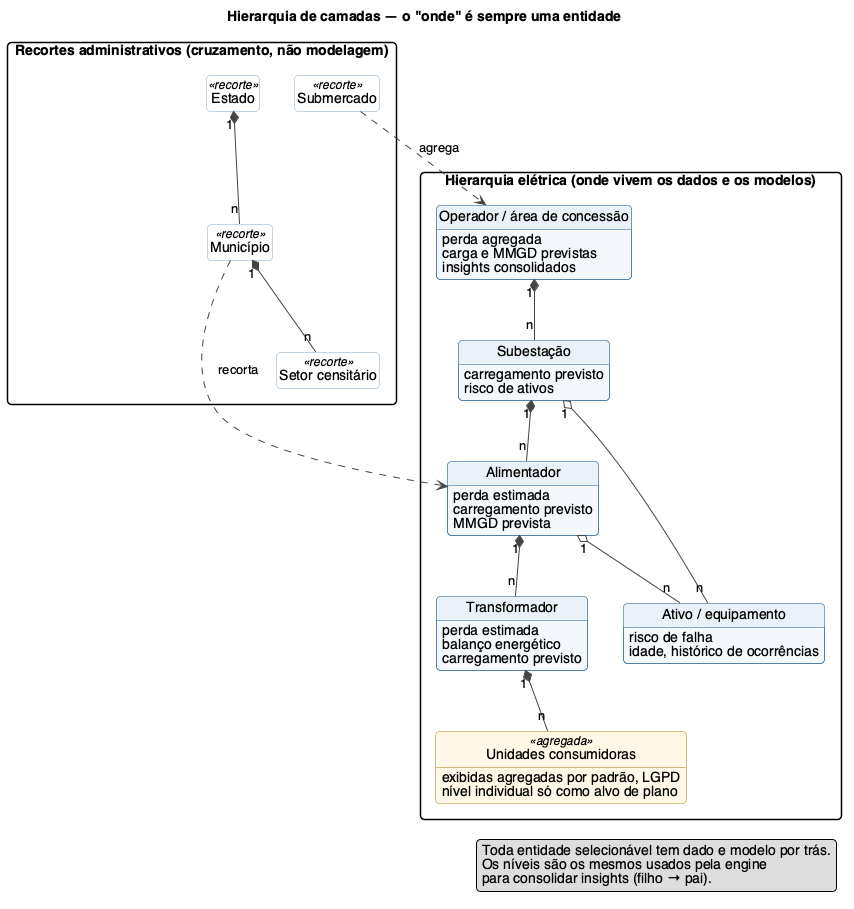
\includegraphics[width=0.82\textwidth]{hierarquia-camadas.png}
\caption{Hierarquia de camadas. A hierarquia elétrica é onde vivem os dados e
os modelos; os recortes administrativos servem para cruzar informação.}
\label{fig:hierarquia}
\end{figure}

Essa escolha tem três consequências:
\begin{itemize}
  \item \textbf{nenhuma seleção é inválida}: tudo o que pode ser escolhido tem
    dado e modelo por trás;
  \item \textbf{tela e engine falam a mesma língua}: os níveis da hierarquia
    são os mesmos que a engine usa para consolidar insights (muitos
    transformadores viram um insight no alimentador);
  \item \textbf{o ponto de partida depende do cliente}: numa distribuidora o
    mapa abre na área de concessão; num gerador, na carteira de parques.
\end{itemize}

\paragraph{Gestos de seleção.}
\begin{enumerate}
  \item \textbf{Clicar} numa entidade de uma camada.
  \item \textbf{Descer ou subir} na hierarquia, com trilha de navegação
    (\emph{Distribuidora › SE Centro › AL-04 › T-1183}).
  \item \textbf{Buscar} por nome ou código.
  \item \textbf{Filtrar por atributo}: ``alimentadores com perda estimada
    acima de 15\%''. O conjunto resultante vira a seleção. É o substituto do
    desenho livre: seleciona-se muita coisa de uma vez por critério, não por
    traço.
  \item \textbf{Selecionar várias} entidades para comparar ou incluir num
    plano.
\end{enumerate}

\subsection{Gestos de saída}

\begin{table}[H]
\centering
\caption{Gestos de saída. Os gestos 1, 2, 3, 5 e 7 fecham o ciclo completo de
valor e formam o MVP.}
\begin{tabularx}{\textwidth}{c l L c}
\toprule
& \textbf{Gesto} & \textbf{Saída} & \textbf{Fase} \\
\midrule
1 & abrir a plataforma & feed de insights da área, sem nenhum input & MVP \\
2 & clicar num insight & mapa vai à entidade e liga as camadas que sustentam
  o achado & MVP \\
3 & selecionar uma entidade & diagnóstico no painel da entidade & MVP \\
4 & perguntar em texto livre & resposta desenhada no mapa & V2 \\
5 & pedir uma decisão & plano de ação (alvos, rotas, valor esperado) sob a
  restrição informada & MVP \\
6 & simular cenário & ``e se a MMGD crescer 30\%?'': alimentadores que
  saturam & V2 \\
7 & registrar resultado & rótulo para o próximo ciclo; insight passa a
  resolvido & MVP \\
\bottomrule
\end{tabularx}
\end{table}

A pergunta em texto livre fica para depois de propósito. Ela impressiona em
demonstração, mas o valor diário vem do feed e do plano, e ela depende de uma
engine madura para não se tornar um chat que inventa respostas.

% ===========================================================================
\section{A tela}
% ===========================================================================

A figura~\ref{fig:mockup} mostra a tela principal no estado de diagnóstico,
depois de o usuário seguir um insight do feed. Os dados são fictícios.

\begin{figure}[H]
\centering
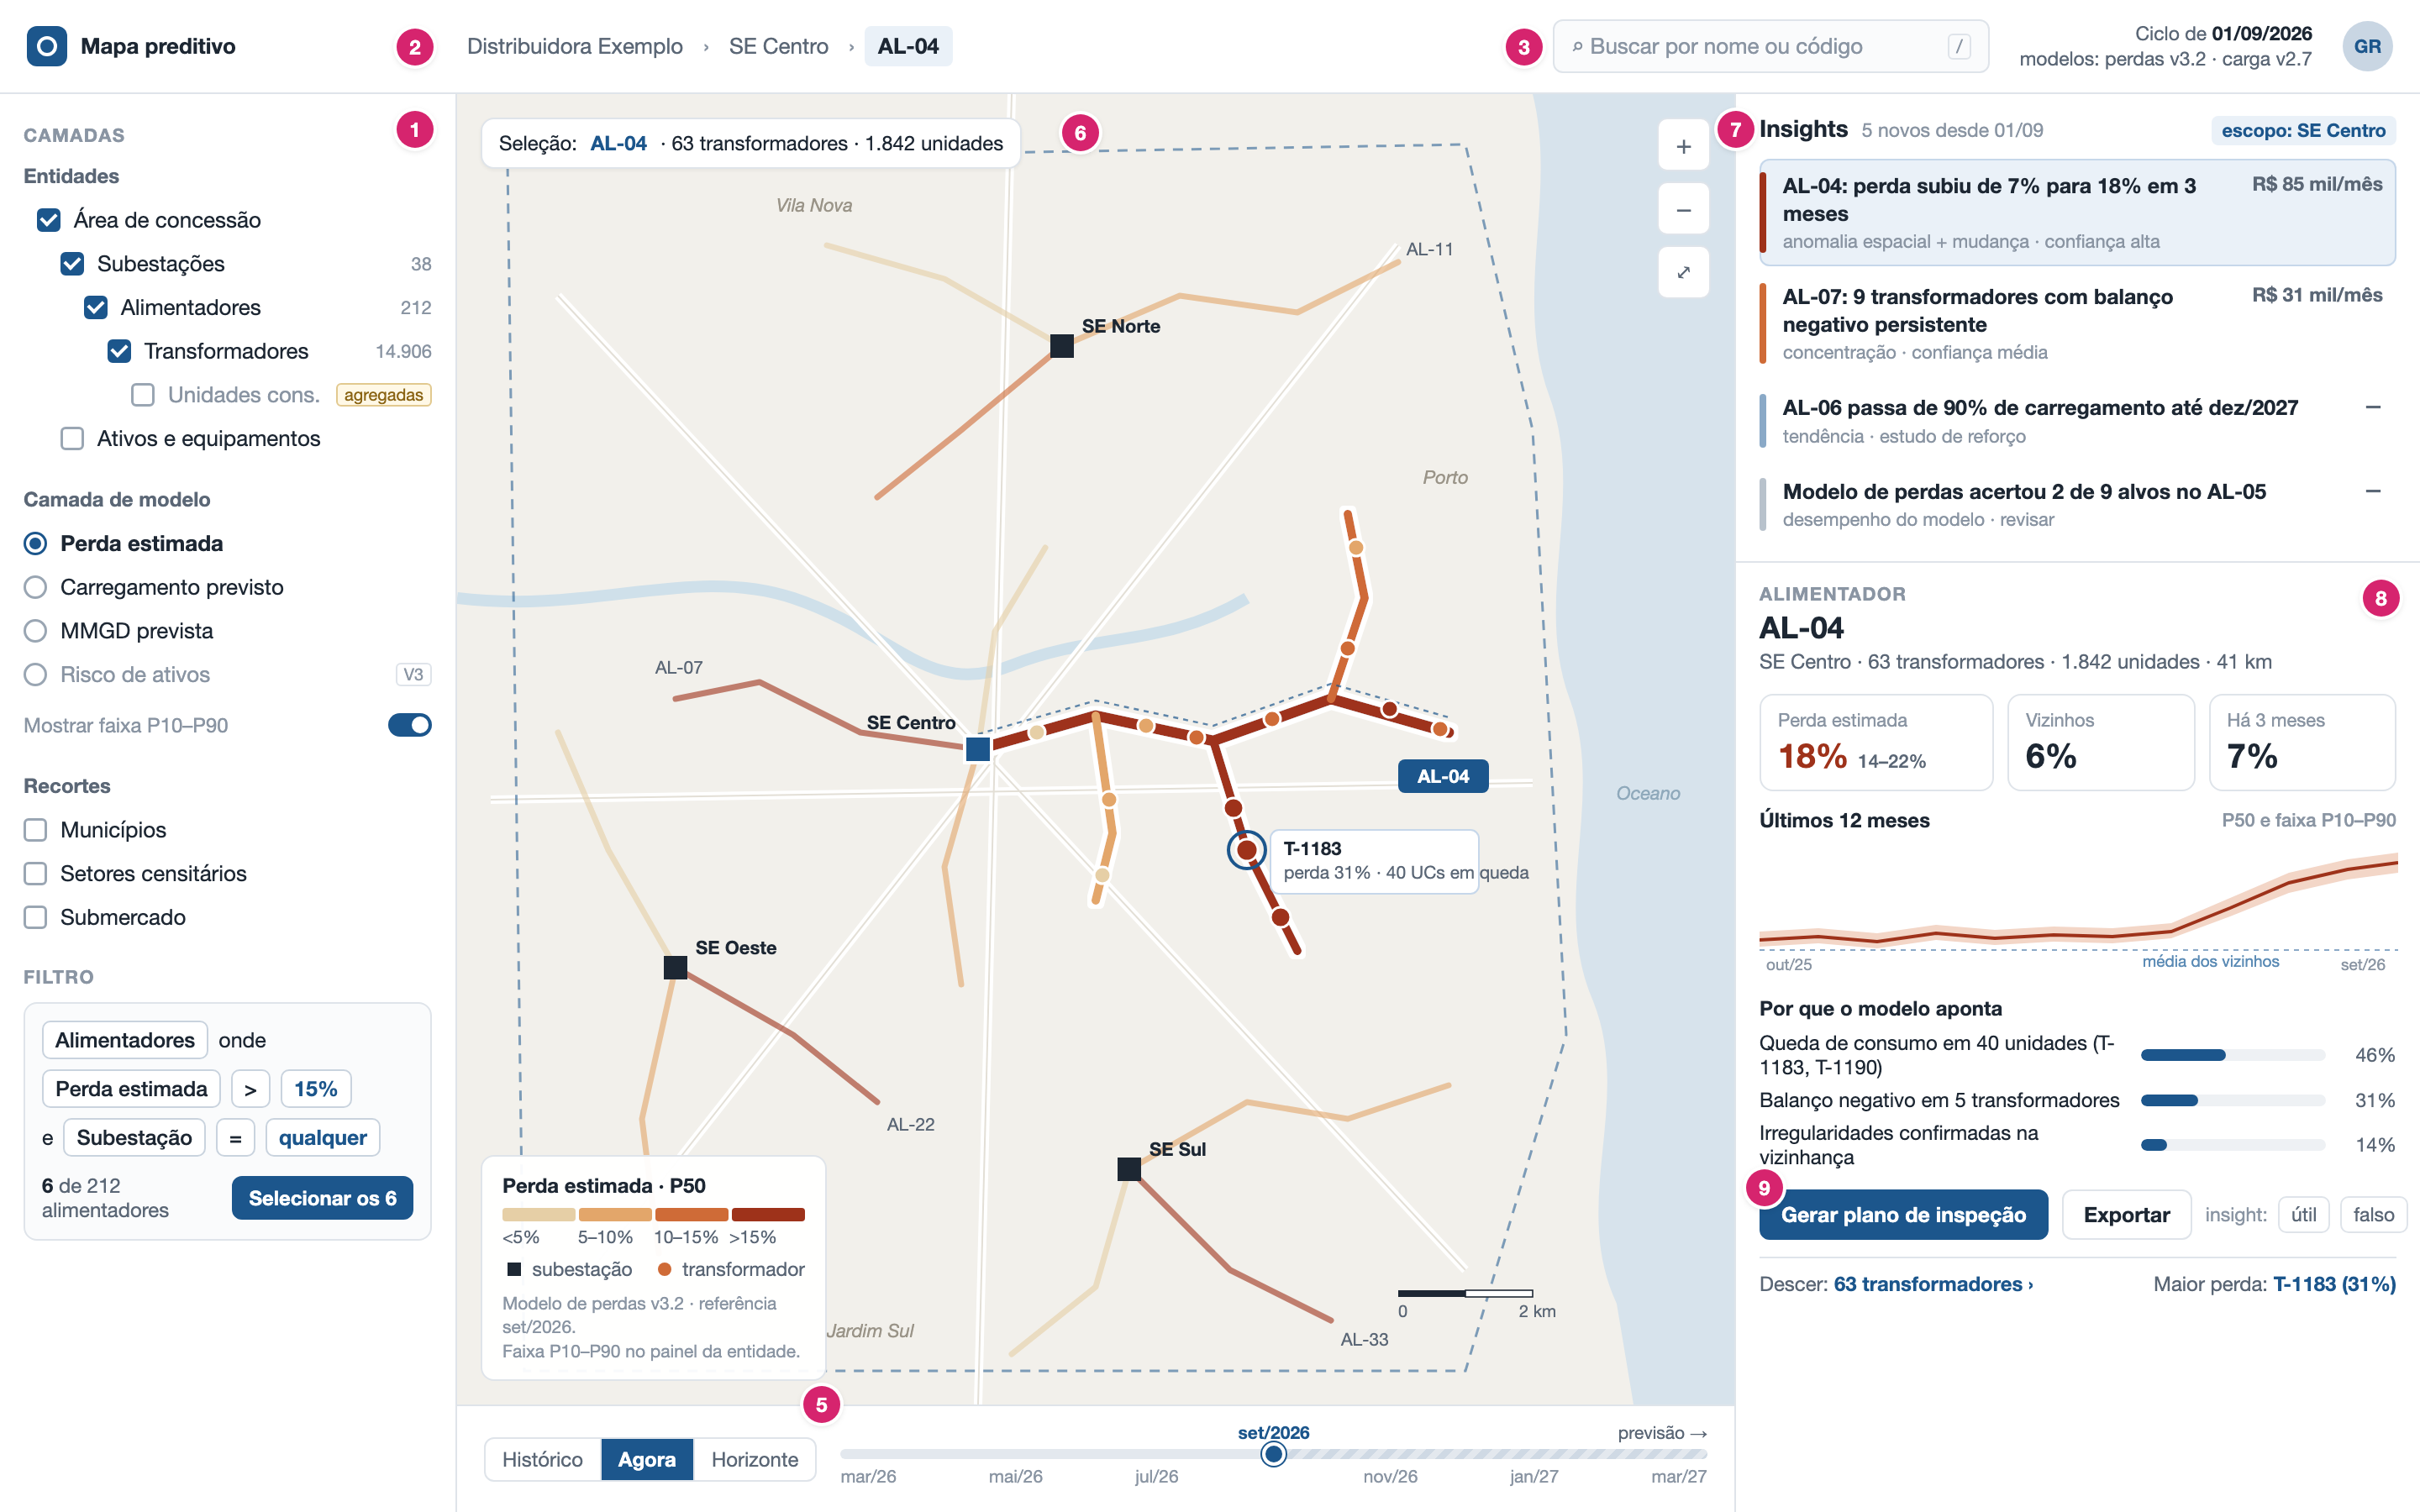
\includegraphics[width=\textwidth]{mockup-diagnostico.png}
\caption{Tela principal, estado de diagnóstico de um alimentador.}
\label{fig:mockup}
\end{figure}

\begin{description}[leftmargin=2em,labelwidth=1.6em]
  \item[\marca{1}] \textbf{Camadas.} Entidades em hierarquia (com contagem),
    a camada de modelo ativa (uma por vez, para que a cor tenha um só
    significado), a exibição da faixa de incerteza e os recortes
    administrativos. Unidades consumidoras aparecem sempre agregadas (R8).
  \item[\marca{2}] \textbf{Trilha.} Onde o usuário está na hierarquia; cada
    nível é clicável para subir.
  \item[\marca{3}] \textbf{Busca} por nome ou código de qualquer entidade.
  \item[\marca{4}] \textbf{Filtro por atributo.} Monta a condição sobre a
    camada e transforma o resultado em seleção.
  \item[\marca{5}] \textbf{Tempo.} Histórico, agora ou horizonte de previsão;
    a parte hachurada é previsão.
  \item[\marca{6}] \textbf{Mapa.} Alimentadores coloridos pela camada ativa
    (P50), a seleção destacada, os transformadores da seleção e o rótulo do
    transformador que mais pesa no diagnóstico. A legenda informa o modelo, a
    versão e a data de referência (R2).
  \item[\marca{7}] \textbf{Feed de insights}, restrito ao escopo da seleção e
    ranqueado por valor. O insight aberto fica marcado.
  \item[\marca{8}] \textbf{Painel da entidade.} Valor com faixa P10--P90,
    comparação com vizinhos e com o passado, série de 12 meses, variáveis que
    mais pesaram e atalho para descer na hierarquia.
  \item[\marca{9}] \textbf{Ação.} Gerar plano de inspeção, exportar e avaliar
    o insight (útil ou falso).
\end{description}

Ao pedir o plano, o painel da entidade dá lugar ao plano
(figura~\ref{fig:plano}): o usuário informa a restrição e a plataforma devolve
os alvos, as rotas por equipe, o valor esperado com faixa e a comparação com o
método atual. Parte dos alvos é reservada para exploração, para corrigir o
viés de seleção discutido no documento de visões.

\begin{figure}[H]
\centering
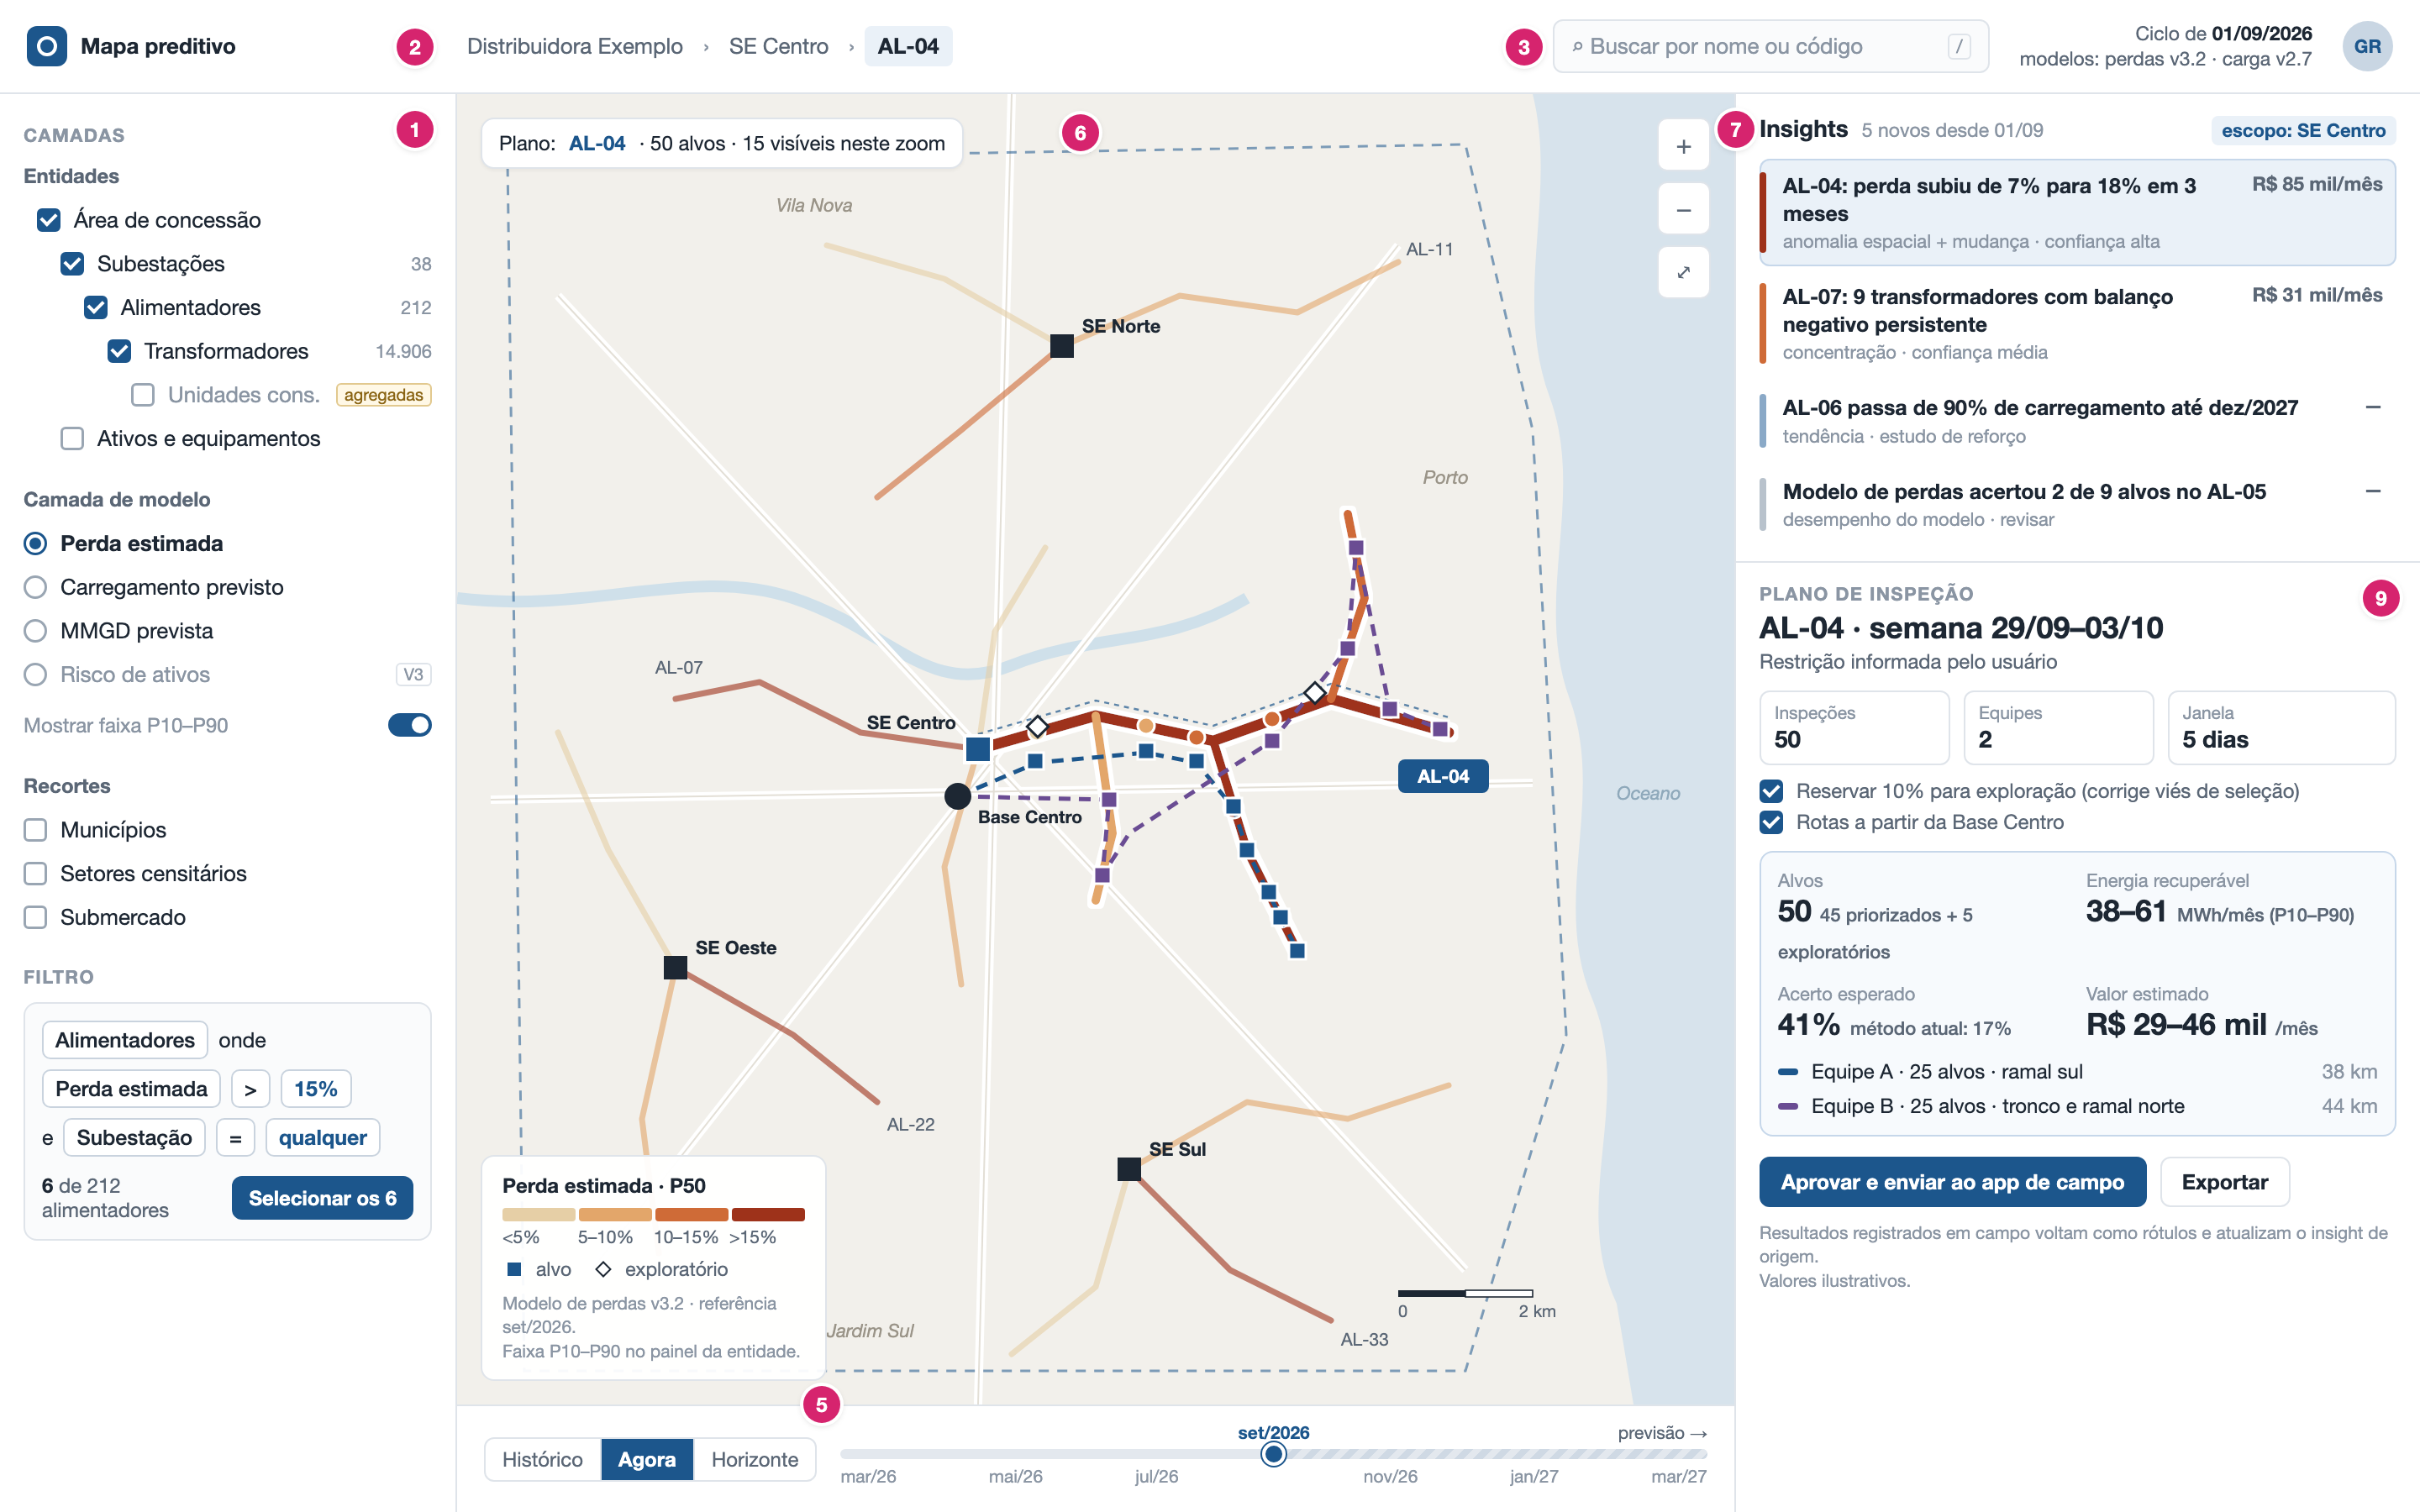
\includegraphics[width=\textwidth]{mockup-plano.png}
\caption{Estado de plano: alvos priorizados e exploratórios, rotas por equipe,
restrição informada e valor esperado.}
\label{fig:plano}
\end{figure}

% ===========================================================================
\section{Engine de análise}
\label{sec:engine}
% ===========================================================================

\subsection{O que é um insight}

Um insight é um achado \emph{calculado} a partir das camadas. Para ser
publicado, precisa ter todos os campos abaixo; sem comparação e sem ação, é
apenas a legenda de uma camada.

\begin{table}[H]
\centering
\caption{Campos obrigatórios de um insight.}
\begin{tabularx}{\textwidth}{l L}
\toprule
\textbf{Campo} & \textbf{Exemplo} \\
\midrule
Onde (entidade) & alimentador AL-04 \\
O quê (métrica e magnitude) & perda estimada de 18\% \\
Comparado com & vizinhos: 6\%; o próprio AL-04 há 3 meses: 7\% \\
Incerteza & P10--P90: 14--22\% \\
Por quê & queda de consumo em 40 unidades; balanço negativo em 5
  transformadores \\
Ação sugerida & plano de inspeção sobre os alvos do topo \\
Valor & cerca de R\$~85 mil por mês recuperáveis \\
\bottomrule
\end{tabularx}
\end{table}

\subsection{Detectores}

\begin{enumerate}
  \item \textbf{Anomalia espacial}: entidade muito diferente das vizinhas
    (estatística espacial local, como LISA ou Getis--Ord).
  \item \textbf{Tendência e limiar}: trajetória prevista cruza um limite
    (``passa de 90\% de carregamento até dez/2027'').
  \item \textbf{Mudança entre ciclos}: o que mudou desde a rodada anterior.
  \item \textbf{Concentração}: aglomerados de perda ou de risco.
  \item \textbf{Divergência modelo × registro}: dado cadastrado que a física
    ou o modelo tornam implausível.
  \item \textbf{Desempenho do próprio modelo}: onde o modelo tem errado. É o
    insight que sustenta a confiança nos demais.
\end{enumerate}

\begin{figure}[H]
\centering
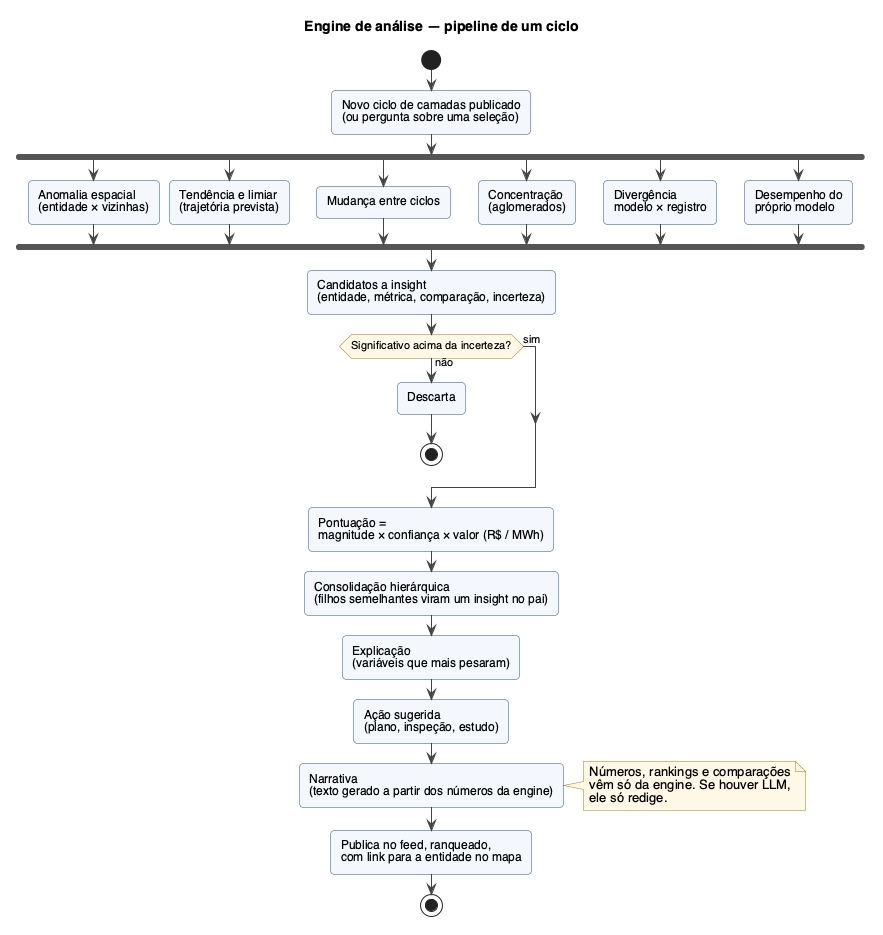
\includegraphics[width=0.78\textwidth]{engine-insights.png}
\caption{Pipeline da engine em um ciclo.}
\label{fig:engine}
\end{figure}

\subsection{Regras de desenho}

\begin{itemize}
  \item \textbf{Todo insight é clicável no mapa.} Abrir um insight leva à
    entidade com as camadas que o sustentam ligadas; feed e mapa são uma
    interface só.
  \item \textbf{Números vêm só da engine.} Se houver um modelo de linguagem,
    ele redige o texto a partir dos números calculados; nunca calcula,
    ranqueia ou compara.
  \item \textbf{Consolidar é obrigatório.} Achados semelhantes em entidades
    irmãs viram um insight no nível pai. A fadiga de alertas, já apontada
    como risco na visão de saúde de ativos, vale igualmente para insights.
  \item \textbf{Significância antes de pontuação.} Um achado que não se
    distingue da incerteza do modelo não é publicado.
\end{itemize}

\subsection{Ciclo de vida}

\begin{figure}[H]
\centering
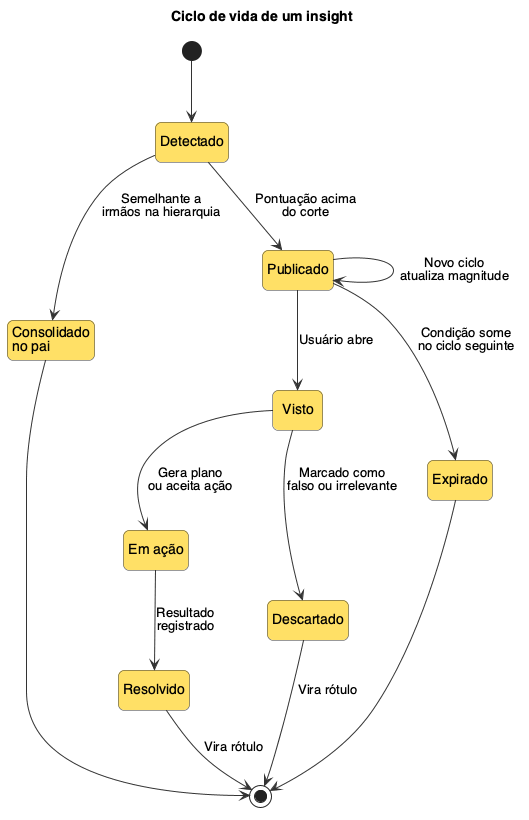
\includegraphics[width=0.55\textwidth]{ciclo-insight.png}
\caption{Ciclo de vida de um insight. Resolvidos e descartados viram rótulos.}
\label{fig:ciclo}
\end{figure}

% ===========================================================================
\section{Arquitetura}
% ===========================================================================

\begin{figure}[H]
\centering
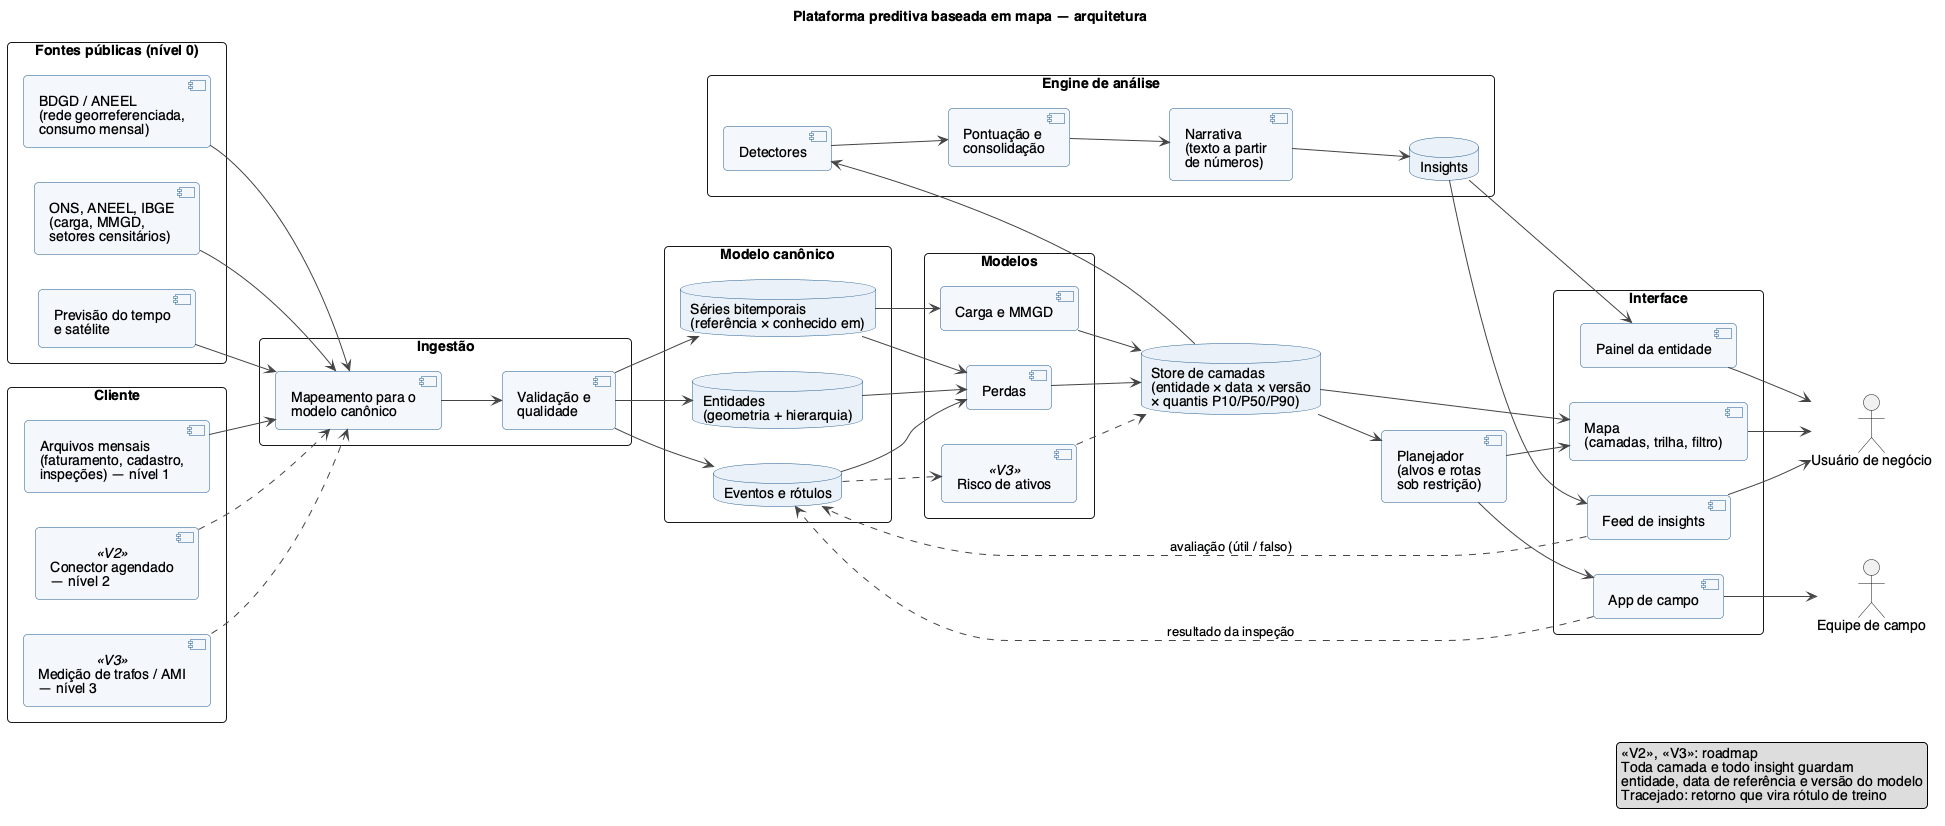
\includegraphics[width=\textwidth]{arquitetura-mapa.png}
\caption{Arquitetura: das fontes ao mapa e ao feed. Tracejado indica roadmap
e o retorno que vira rótulo de treino.}
\label{fig:arquitetura}
\end{figure}

\subsection{Modelo canônico}

Qualquer que seja a origem, a ingestão converte os dados para quatro formas:

\begin{enumerate}
  \item \textbf{Entidade com geometria} e posição na hierarquia: a chave de
    tudo.
  \item \textbf{Série temporal} de uma entidade, com data de referência e
    data em que o dado ficou conhecido (bitemporal, para evitar vazamento).
  \item \textbf{Evento}: inspeção, falha, manutenção, curtailment.
  \item \textbf{Rótulo}: o resultado de um evento.
\end{enumerate}

Integrar um cliente novo é escrever o mapeamento dos arquivos dele para essas
quatro formas: configuração, não código.

\subsection{Entrada de dados por níveis}

\begin{table}[H]
\centering
\caption{Níveis de entrada de dados. O ciclo de faturamento é mensal, então
o MVP não precisa de streaming.}
\begin{tabularx}{\textwidth}{c L L}
\toprule
\textbf{Nível} & \textbf{Entrada} & \textbf{O que habilita} \\
\midrule
0 & só dados públicos (BDGD, ONS, ANEEL, IBGE, previsão do tempo) & mapa da
  rede e camadas estimadas; demonstração e piloto sem dado do cliente \\
1 & arquivos mensais do cliente (faturamento, cadastro, inspeções) & modelo
  de perdas por transformador e unidade; planos de inspeção (\textbf{MVP}) \\
2 & conector agendado (banco, SFTP, API) & atualização sem trabalho manual \\
3 & medição contínua (transformadores, medição inteligente) & balanço quase
  em tempo real; previsão intradiária \\
\bottomrule
\end{tabularx}
\end{table}

\begin{nota}
\textbf{Atalho parcial.} A BDGD é gerada pela própria distribuidora a partir
dos seus sistemas. Nos arquivos abertos, os códigos de alimentador,
transformador e pontos de conexão parecem operacionais, então o dado do
cliente tende a se ligar ao mapa \emph{pela rede} sem geocodificação. Já a
unidade consumidora vem anonimizada (hash): ligar \emph{por unidade} exige a
tabela de correspondência da distribuidora. A BDGD pública também chega com 8
a 20 meses de defasagem, então serve para montar a rede e o piloto, e o dado
mensal vem do cliente (nível 1). Detalhes em \emph{Features de energia}.
\end{nota}

% ===========================================================================
\section{Casos de uso e sessão típica}
% ===========================================================================

\begin{figure}[H]
\centering
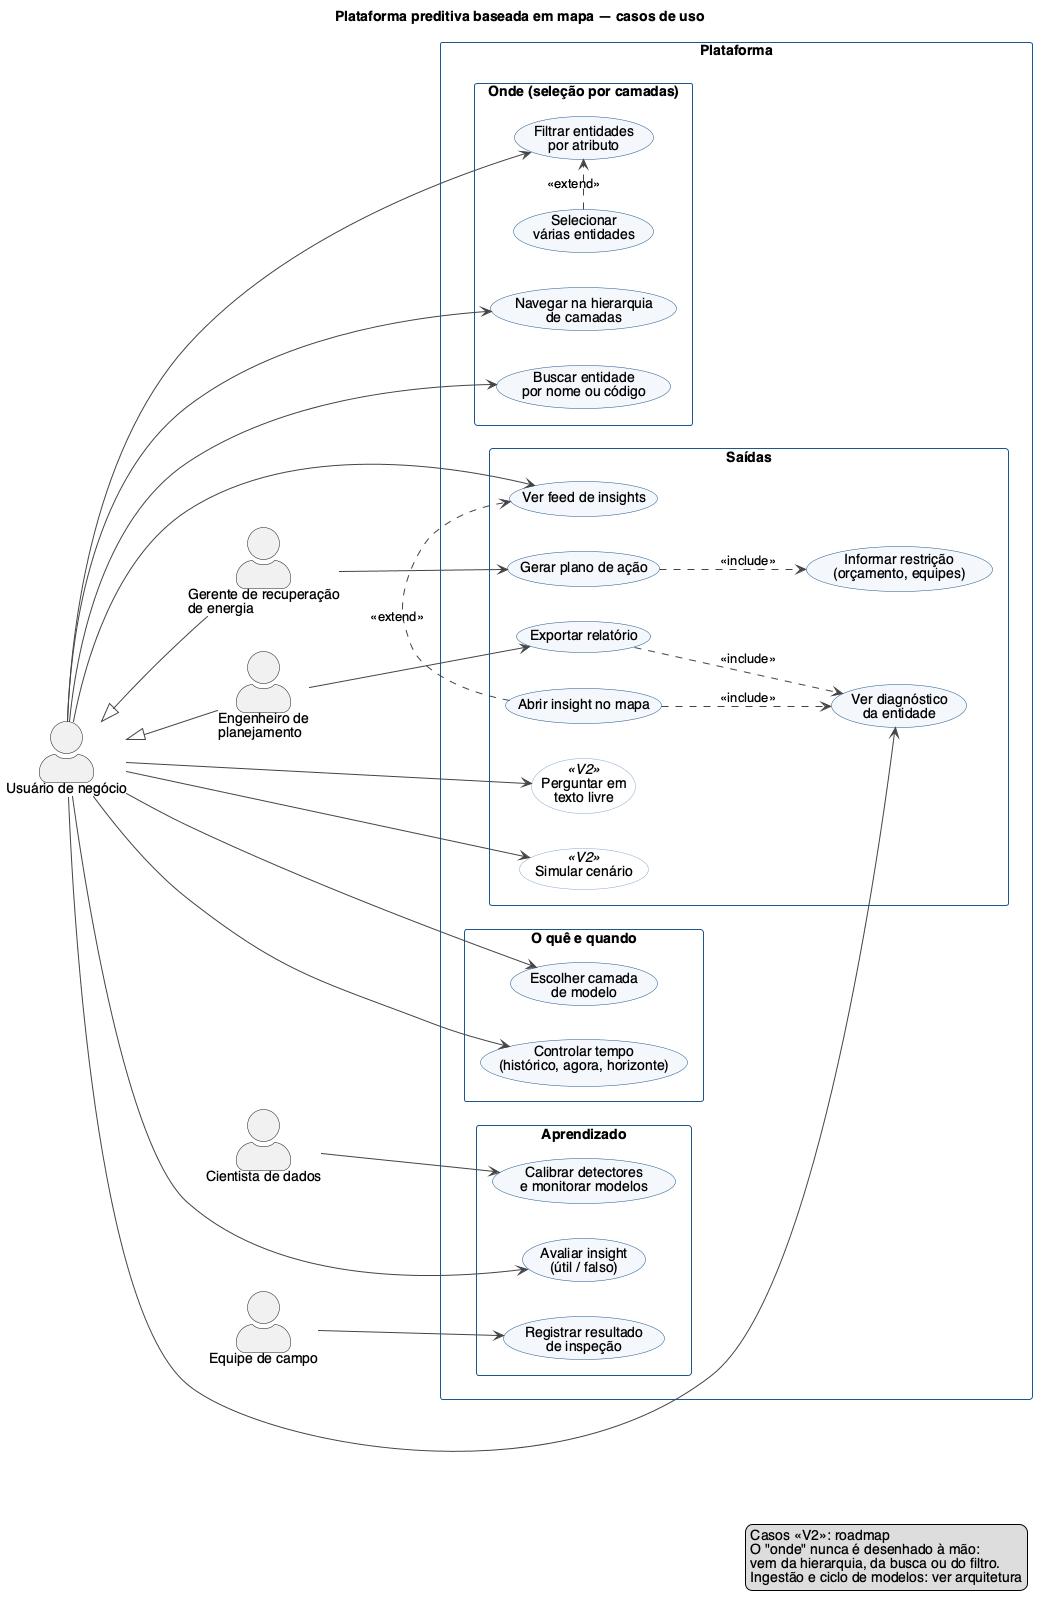
\includegraphics[width=0.72\textwidth]{casos-de-uso-mapa.png}
\caption{Casos de uso agrupados por parte do input e por tipo de saída.}
\label{fig:casos}
\end{figure}

\begin{figure}[H]
\centering
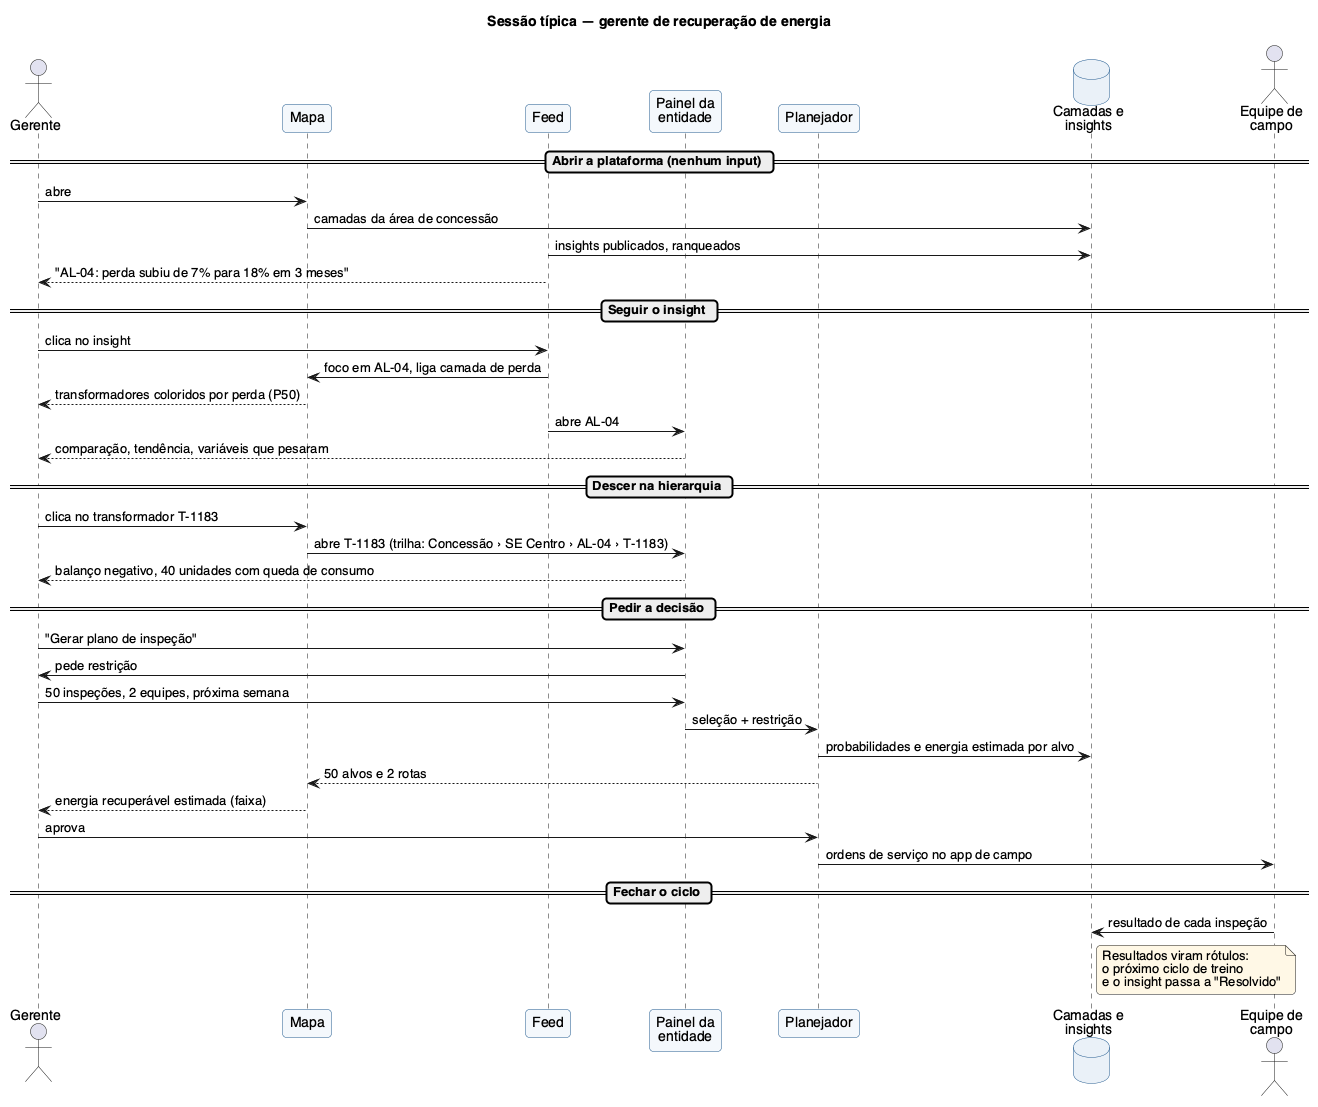
\includegraphics[width=\textwidth]{sessao-usuario.png}
\caption{Sessão típica de um gerente de recuperação de energia: do feed ao
plano e ao resultado em campo.}
\label{fig:sessao}
\end{figure}

% ===========================================================================
\section{Escopo do MVP e evolução}
% ===========================================================================

\paragraph{MVP.}
\begin{itemize}
  \item Hierarquia elétrica a partir da BDGD da distribuidora cliente.
  \item Camadas: perda estimada por transformador e alimentador.
  \item Engine com os detectores de anomalia espacial, mudança entre ciclos e
    desempenho do modelo.
  \item Gestos 1, 2, 3, 5 e 7: feed, abrir insight, diagnóstico, plano de
    inspeção e registro de resultado.
  \item Entrada de dados de nível 1 (arquivos mensais).
\end{itemize}

\paragraph{Evolução.}
\begin{itemize}
  \item \textbf{V2}: camadas de carregamento e MMGD previstos por alimentador;
    detectores de tendência e concentração; pergunta em texto livre e
    simulação de cenário; conector agendado.
  \item \textbf{V3}: risco de ativos; medição contínua; detector de
    divergência modelo × registro.
  \item \textbf{V4}: pontos quentes de operação (copiloto), se validado.
\end{itemize}

% ===========================================================================
\section{Riscos}
% ===========================================================================

\begin{itemize}
  \item \textbf{Fadiga de insights}: feed longo e medíocre faz o usuário
    parar de olhar. Mitigação: significância, consolidação e corte por valor.
  \item \textbf{Texto que inventa números}: mitigado pela regra de que números
    vêm só da engine.
  \item \textbf{Viés de seleção nos rótulos}: inspeções passadas não são
    aleatórias. Mitigação: fração exploratória em todo plano.
  \item \textbf{LGPD e sensibilidade social}: indicação de irregularidade não
    é prova; exibição agregada por padrão e monitoramento de viés geográfico.
  \item \textbf{Qualidade dos dados públicos}: na BDGD, a energia da MMGD
    se comporta como injeção, não geração, a potência instalada mistura kW e
    W, e a mesma coluna vem em kWh numa distribuidora e em MWh em outra. A
    perda não técnica da BDGD é rateio contábil. Toda camada derivada precisa
    declarar a normalização usada.
\end{itemize}

% ===========================================================================
\section{Questões em aberto}
\label{sec:abertas}
% ===========================================================================

\begin{enumerate}
  \item \textbf{Cliente-alvo.} Distribuidora (hipótese deste documento) ou
    gerador e comercializadora. Muda a hierarquia de camadas, os modelos do
    MVP e a métrica de valor; a engine e o modelo de interação permanecem.
  \item \textbf{Códigos da BDGD × códigos internos.} Confirmar com um cliente
    que os códigos de rede coincidem e se ele fornece a correspondência do
    código anonimizado das unidades.
  \item \textbf{Corte de publicação.} Quantos insights por ciclo o usuário
    aceita ler; define o limiar de pontuação.
  \item \textbf{Nome do produto.} ``Mapa preditivo'' é nome de trabalho.
\end{enumerate}

\end{document}
